\documentclass[12pt, titlepage]{article}
\usepackage{cite}
\usepackage{amsbsy}
\usepackage[a4paper, total={6in, 8in}, left=40mm, top = 20mm, bottom = 20mm]{geometry}
\usepackage{graphicx}
\usepackage{multirow}
\usepackage{booktabs}
\usepackage{wasysym}
\usepackage{float}
\usepackage{setspace}
\usepackage[euler]{textgreek}
\usepackage{textcomp}
\usepackage{amssymb}
\usepackage{caption} 
\usepackage{lscape}
\usepackage{pdfpages}
\usepackage{fancyref}
\usepackage[round]{natbib}

\captionsetup[table]{skip=10pt}
\doublespacing

\setlength{\parskip}{1em}
\setlength{\parindent}{4em}
\graphicspath{ {C:/Users/sra2g13/Documents/PhD/GitHub/mytophid-ears/Outputs/Graphs/} }
\title{Field metabolic rates of Scotia Sea myctophids (family Myctophidae)\\
\large{Confirmation Report}}
\author{Sarah R. Alewijnse}     

\begin{document}
\maketitle
\tableofcontents
\pagebreak

\section{Abstract}

Myctophids (family Myctophidae) are an important part of the biological carbon pump in the oceans.
Estimating the magnitude of their contribution to the biological carbon pump requires knowledge of their field metabolic rate; the time-averaged rate at which they use energy while free-ranging in their natural environment.
Here, I present the first estimates of relative field metabolic rate for six species of myctophids (\textit{Electrona antarctica, E. carlsbergi, Gymnoscopelus braueri, G. nicholsi, Protomyctophum bolini} and \textit{Krefftichthys anderssoni}) from the Scotia Sea, using a novel proxy for field metabolic rate based on otolith \textdelta \textsuperscript{13}C.
Contrary to metabolic theory, differences among species were the most important drivers of variation in metabolic rate, rather log body mass and temperature.
I explore why field metabolic rate is different among these species by comparing the ecology and life history characteristics of the six species.
Additionally, estimates of field metabolic rate did not positively correlate with estimates of resting metabolic rate, suggesting that current calcuations of myctophid contribution to the biological carbon pump in the Scotia Sea are inaccurate.

\pagebreak
\section{Introduction}

Mesopelagic fishes (those living in the mesopelagic zone, between 150-1000m) are an important component of the ocean biological carbon pump \citep{Anderson2018, Trueman2014}.
They oftern undertake diel vertical migrations, swimming from depth to surface waters at night to feed on zooplankton, before returning to the deep prior to daybreak.
By completing this diel vertical migration, migratory mesopelagic fishes transport carbon away from the surface waters, and export this carbon in the mesopelagic through respiration, excretion and mortality. 
Non-migratory mesopelagic fishes also contribute to the biological carbon pump by consuming migrating zooplankton in the mesopelagic zone \citep{Davison2013}.
The deeper carbon is transported in the ocean, the longer it is prevented from returing to the surface and fluxing with the atmosphere \citep{Passow2012}.
Interest in harvesting mesopelagic fishes is increasing, driven by a growing requirement for fishmeal to sustain aquaculture \citep{Catul2011, Davison2013, StJohn2016}.
To fully understand the potential impact of harvesting mesopelagic fishes, we must first quantify the role they play in the biological carbon pump.

Myctophids (family Myctophidae) are the dominant mesopelagic fishes in the Scotia Sea, a highly productive area of the Southern Ocean. \citep{Catul2011, Collins2012}.
Scotia Sea myctophids are estimated to contribute 0.05 to 0.28 mg C m\textsuperscript{-2} d\textsuperscript{-1} to active carbon flux, equivalent to 9 to 47\% of gravitational particulate organic carbon flux in the same area \citep{Belcher2019}.
This estimate is obtained by estimating myctophid metabolic rate from the regression equation:

\begin{equation}
\label{equ:RMR}
Ln(RMR_{W}) = a + b_{W} \times Ln(WM) + b_{T} \times T
\end{equation}

\noindent Where $RMR_{W}$ is wet mass-specific resting metabolic rate (\textmu l O\textsubscript{2} mg WM\textsuperscript{-1} h\textsuperscript{-1}), and $T$ is temperature (\textdegree C).

This equation was parameterised based on five studies of myctophid respiration rate, \citep{Ariza2015, Donnelly1988, Ikeda1989, Torres1979, Torres1988a}
 measured through either respirometry or electron transport system enzyme activity (ETS), both of which are less than ideal methods for this group of fishes.
Myctophids are delicate fishes, and are often dead or damaged on landing \citep{Catul2011}.
Consequently, fishes which are subjected to respirometry are likely to be stressed, giving artificially high measures of metabolic rate.
These studies selected the most active fish in a catch, which potentially biases measures towards fish with higher metabolic rates \citep{Torres1988a}.
ETS measures the respiration potential of a sample of tissue, which is then converted to whole organism metabolic rate using a ratio of ETS and respirometry \citep{Ariza2015, Cammen1990, Ikeda1989}.
No direct calibrations between ETS and oxygen consumption are available for myctophids, which may lead to inaccurate estimates of metabolic rate.

Both of these methods measure or estimate resting metabolic rate (RMR), the minimum metabolic rate of a resting organism, in a post-absorptive state \citep{Treberg2016}.
RMR is a less useful measurement of metabolic rate in the context of the biological carbon pump than field metabolic rate (FMR).
FMR is the time-averaged energy expenditure of an organism free-ranging in its natural habitat \citep{Treberg2016}.
FMR includes energy expended on basal costs, as with RMR, but also incorporates the thermic effect of food (also called specific dynamic action), as well as energy used for growth, reproduction, movement and excretion \citep{Chung2019a, Chung2019b, Treberg2016}.

In this study I used a novel method to calculate $M$ value, a proxy for mass-specific FMR \citep{Chung2019b}.
Otoliths are calcium carbonate structures found in the inner ears of fishes.
The carbon in the otolith comes from the surrounding endolymph, which itself comes from carbon in the blood \citep{Campana1998, Solomon2006}.
Blood carbon comes from two sources: metabolic (dietary) carbon, produced during cellular respiration, and dissolved inorganic carbon from the surrounding water.
These two sources of carbon are isotopically distinct, with dissolved inorganic carbon having a greater proportion of carbon-13 to carbon-12, than metabolic carbon (\textdelta \textsuperscript{13}C of dissolved inorganic carbon is 15\permil\ more positive \textdelta \textsuperscript{13}C of metabolic carbon) \citep{Magozzi2017, Tagliabue2008}.
Fish with relatively higher metabolic rates have higher respiration rates, so produce more metabolic carbon.
As fish regulate the levels of carbonate in their blood, this increase in metabolic carbon is compensated by a decrease in dissolved inorganic carbon, increasing the proportion of metabolic carbon in the blood, meaning (\textdelta \textsuperscript{13}C) in the blood has a more negative value.
Therefore \textdelta \textsuperscript{13}C values of otoliths are a weighted average of \textdelta \textsuperscript{13}C values from metabolic carbon and dissolved inorganic carbon \citep{Chung2019b, Trueman2016}.
If \textdelta \textsuperscript{13}C values are known, the proportion of metabolic carbon ($M$ value) can be calculated, as was done in this study (section \ref{sec:M}).
While this is a novel method, a recent study confirmed that $M$ values and oxygen consumption were positively correlated in cod (\textit{Gadus morhua}), giving empirical support for the use of $M$ as a metabolic proxy \citep{Chung2019a}.

The primary aim of this study is to use $M$ values to compare relative FMR between six species of myctophids common in the Scotia Sea: \textit{Electrona antarctica, E. carlsbergi, Gymnoscopelus braueri, G. nicholsi, Protomyctophum bolini} and \textit{Krefftichthys anderssoni} \citep{Collins2008, Collins2012, Piatkowski1994}.
This study is the first comparison of FMR between species of myctophids to date.

I will also investigate the scaling relationships of $M$ values with body mass and temperature.
According to the metabolic theory of ecology, metabolic rates scale linearly with log body mass and temperature \citep{Brown2004}.
I will examine whether this is the case for FMR by modelling $M$ values as a linear function of log body mass and temperature.
If the metabolic theory is correct, $M$ values should decrease with increasing log body mass, and increase with increasing temperature, both within and between species.
Temperature is obtained from otolith stable isotopes, using \textdelta \textsuperscript{18}O (section \ref{sec:temp}).

Finally, I will compare estimates of mass-specific RMR generated using equation \ref{equ:RMR}, and $M$ values.
As RMR is likely to be a component of FMR, studies predict that these two measures of metabolic rate will be positively correlated. % Degen & Kam - Double check

\pagebreak
\section{Methods}

\subsection{Data Collection}
\label{sec:data}

\subsubsection{Otolith Stable Isotope Analysis}

Otoliths from six species of myctophids from the Scotia Sea were donated by the British Antarctic Survey for this study: \textit{Electrona antarctica} (n = 19), \textit{E. carlsbergi} (n = 17), \textit{Gymnoscopelus braueri} (n = 20), \textit{G. nicholsi} (n = 13), \textit{Krefftichthys anderssoni} (n = 20) and \textit{Protomyctophum bolini} (n = 20).
Due to a labelling error, eight \textit{E. carlsbergi} individuals did not have body mass recorded, and were omitted for all body mass analyses.

Prior to stable isotope analysis, each otolith was cleaned in water, allowed to dry and mounted onto a backing plate (Struers EpoFix resin).
The outer surface of the otolith (100-200 \textmu m depth) was milled using an ESI NewWave Micromill, to ensure that the otolith material deposited most closely to the time of capture was analysed.
Where the otoliths were too small to be milled ($<$1mm diameter - all \textit{K. anderssoni} and some \textit{P. bolini}), they were crushed to obtain powder for stable isotope analysis.
Supplementary analyses (appendix \ref{app:supp}) were run to test whether this caused a significant difference in $M$ values.

\subsubsection{$M$ Values}
\label{sec:M}

A mixing model was used to estimate the proportion of metabolic carbon in the blood, $M$:

\begin{equation}
M = \frac{\delta^{13}C_{oto}-\delta^{13}C_{DIC-SW}}{\delta^{13}C_{diet}-\delta^{13}C_{DIC-SW}} + e_{total}
\end{equation}

\noindent Where $\delta^{13}C_{oto}$ is the \textdelta \textsuperscript{13}C value of the fish's otolith, $\delta^{13}C_{DIC-SW}$ is the value for \textdelta \textsuperscript{13}C of dissolved inorganic carbon (DIC) ingested by the fish through seawater, $\delta^{13}C_{diet}$ is the \textdelta \textsuperscript{13}C of the diet, and $e_{total}$ is the isotopic fractionation from DIC to blood, blood to endolymph, and endolymph to otolith. 
For this study I assumed that $e_{total}$ was invariant across species, and that $M$ values were directly proportional to the percentage of metabolic carbon in the fish's blood \citep{Chung2019b}.

In calculating $M$ values, parameters were allowed to vary across normal and truncated normal \citep{truncnorm} distributions with means, standard deviations, and minimum and maximum values set according to the relevant literature (appendix A).
$\delta^{13}C_{DIC-SW}$ was set using catch location and corrected for the Suess effect (the decrease in \textdelta \textsuperscript{13}C with time, due to anthropogenic carbon dioxide emissions), from the model by \cite{Tagliabue2008}.
$\delta^{13}C_{diet}$ was set using \textdelta \textsuperscript{13}C of phytoplankton (set by catch location) from the model by \cite{Magozzi2017}, trophic levels from \cite{Fishbase}
and the trophic enrichment factor for carbon from \cite{DeNiro1978}.
$e_{total}$ was set to the value from \cite{Solomon2006}.
10,000 random samples were taken from the resulting distribution of $M$ values for each individual.

\subsubsection{Reconstructed Temperature}
\label{sec:temp}

\textdelta \textsuperscript{18}O of otolith aragonite can be used to estimate the ambient temperature experienced by a fish \citep{Thorrold1997, Hoie2004}.
Experienced temperature ($T$) was reconstructed using the following equation:

\begin{equation}
T = \frac{(\delta^{18}O_{oto} - \delta^{18}O_{SW}) - a}{b}
\end{equation}

\noindent Where $\delta^{18}O_{oto}$ is the \textdelta \textsuperscript{18}O of the otolith, $\delta^{18}O_{SW}$ is the \textdelta \textsuperscript{18}O of the ambient seawater, and $a$ and $b$ are parameters, set according to \cite{Hoie2004}. $\delta^{18}O_{SW}$  was set according to \cite{Schmidt1999}, by catch location and depth. 
As with $M$ values, all parameters were allowed to vary across normal and truncated normal distributions (appendix B).

\subsubsection{Estimates of log Mass-Specific Resting Metabolic Rate}

Estimates of log specific resting metabolic rate (RMR) were calculated using equation 1.
Parameters were set according to \cite{Belcher2019} so that $a$ = -1.315(\textpm 0.468), $b_{W}$ = -0.2665 (\textpm 0.0516), and $b_{T}$ = 0.0848(\textpm 0.0108).

\subsection{Statistical Analyses}

All statistical analyses were carried out in R \citep{R}. Hamiltonian Monte Carlo (HMC) models were run in RStan \citep{RStan} using the rethinking package \citep{Rethinking}. Convergence and mixing were checked using effective sample size (N\_eff), \^R, and traceplots (appendix D).

To examine the effect of log body mass and temperature on $M$ values, I modelled estimates of $M$ values as a linear function of log body mass ($W$) and temperature ($T$) in an HMC simulation of 1,000,000 iterations, with 500,000 warmup, a single chain, and a thinning parameter of 1. 
Species was included in the model as a random factor to address the problem of pseudoreplication within species.
This also gave estimates of the mean $M$ value for each species, and allowed me to assess whether $M$ values varied significantly between species.

\begin{center}
\textbf{Model 1 - Body Mass and Temperature}
\\$M_{est, i} \sim Normal(\mu_{i}, \sigma)$
\\$\mu_{i} = a_{1} + b_{W} \times W + b_{T} \times T_{est, i} + a\_Var_{Species}$
\\$M_{obs, i} \sim Normal(M_{est, i}, M_{sd, i})$
\\$T_{obs, i} \sim Normal(T_{est, i}, T_{sd, i})$
\\$a_{1} \sim Normal(0.20, 0.5)$
\\$b_{W} \sim Normal(0, 0.5)$
\\$b_{T} \sim Normal(0, 0.5)$
\\$a\_Var_{Species} \sim Normal(0, \sigma_{Species})$
\\$\sigma_{Species} \sim Cauchy(0, 1)$
\\$\sigma \sim Cauchy(0, 0.1)$
\label{mod:WT}
\end{center}

Within species, I investigated the relationship between $M$ values and log body mass and temperature using the following HMC simulations of 10,000 iterations, with 1000 warmup, 4 chains, and a thinning parameter of 1.

\begin{center}
\textbf{Model 2 - Temperature} (variable n)
\\$M_{est, i} \sim Normal(\mu_{i}, \sigma)$
\\$\mu_{i} = a + b_{T} \times T_{est, i}$
\\$M_{obs, i} \sim Normal(M_{est, i}, M_{sd, i})$
\\$T_{obs, i} \sim Normal(T_{est, i}, T_{sd, i})$
\\$a \sim Normal(0.25, 1)$
\\$b_{T} \sim Normal (0, 1)$
\\$\sigma \sim Cauchy(0, 1)$
\end{center}

\begin{center}
\textbf{Model 3 - Body Mass} (variable n)
\\$M_{est, i} \sim Normal(\mu_{i}, \sigma)$
\\$\mu_{i} = a + b_{W} \times W$
\\$M_{obs, i} \sim Normal(M_{est, i}, M_{sd, i})$
\\$a \sim Normal(0.25, 1)$
\\$b_{W} \sim Normal (0, 1)$
\\$\sigma \sim Cauchy(0, 1)$
\end{center}

\pagebreak
I generated estimates of log mass-specific RMR using equation 1, inputting body mass, and temperature calculated for \textdelta \textsuperscript{18}O.
I modelled estimates of $M$ values ($M$) as a linear function of estimates of log mass-specific RMR ($RMR$), using an HMC simulation of 10,000 iterations with 1000 warmup, 4 chains and a thinning parameter of 1.

\begin{center}
\textbf{Model 4 - Resting Metabolic Rate} (n = 100)
\\$M_{est, i} \sim Normal(\mu_{i}, \sigma)$
\\$\mu_{i} = a + b \times RMR_{est, i}$
\\$M_{obs, i} \sim Normal(M_{est, i}, M_{sd, i})$
\\$RMR_{obs, i} \sim  Normal(RMR_{est, i}, RMR_{sd , i})$
\\$a \sim Normal(0.2, 1)$
\\$b \sim Normal(0, 10)$
\\$\sigma \sim Cauchy(0.1, 1)$
\end{center}

\pagebreak
\section{Results}

\subsection{Relative Field Metabolic Rate Between Species}

There was substantial overlap in $M$ values between the six species of myctophids (figure \ref{fig:dens}).
\textit{K. anderssoni} ($M$ = 0.2468 \textpm 0.0244) \textit{E. antarctica} ($M$ = 0.2312 \textpm 0.0228) and \textit{G. braueri} ($M$ = 0.2201 \textpm 0.0235) had the highest estimates of species means of $M$ , followed by \textit{E. carlsbergi} ($M$ = 0.1959 \textpm 0.0237) and \textit{P. bolini} ($M$ = 0.1888 \textpm 0.0241).
\textit{G. nicholsi} with had the lowest estimates for $M$ ($M$ = 0.1548 \textpm 0.0257) (table \ref{tab:WT}).

\begin{figure}[H]
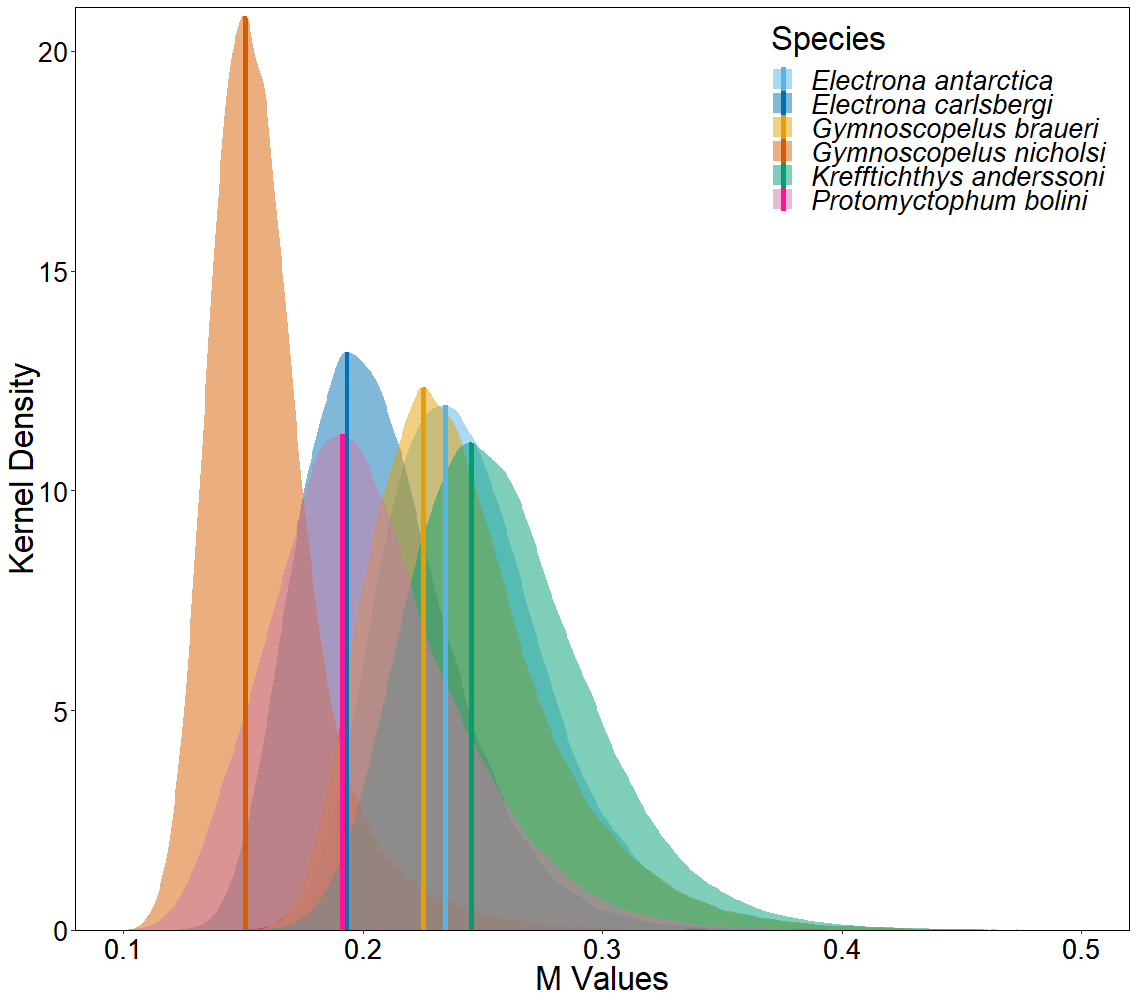
\includegraphics[width=\linewidth]{Density.png}
\caption{Kernel density of 10,000 estimates of $M$ (a proxy for FMR) per individual fish, across 108 individuals, combined and grouped by six species. Maximum density of the distribution of each species is indicated by the solid lines.}
\label{fig:dens}
\end{figure}

\begin{table}[H]
\begin{center}
\caption{Posterior predictions of parameters for $M$ values as a function of log body mass and reconstructed temperature (model 1), with convergence and mixing diagnostics: number of effective samples (N\_eff) and \^R. ELN = \textit{Electrona antarctica}, ELC = \textit{E. carlsbergi}, GYR = \textit{Gymnoscopelus braueri}, GYN = \textit{G. nicholsi}, KRA = \textit{Krefftichthys anderssoni}, PRM = \textit{Protomyctophum bolini}.}
\label{tab:WT}

\def\arraystretch{1.5}
  \begin{tabular}{ | l | l | l | l | l |}
    \hline
    \textbf{Parameter} & Mean & SD & N\_eff & \^R \\ \hline
    $a_{1}$ & 0.2066 & 0.0244 & 12997 & 1.00 \\ \hline
   $b_{W}$ & 0.0015 & 0.0137 & 15468 & 1.00\\ \hline
    $b_{T}$ & -0.002 & 0.0022 & 14438 & 1.00 \\ \hline
    $a\_Var_{ELN}$ & 0.0246 & 0.0228 & 18448 & 1.00 \\ \hline
    $a\_Var_{ELC}$ & -0.0107 & 0.0237 & 11154 & 1.00 \\ \hline
    $a\_Var_{GYR}$ & 0.0135 & 0.0235 & 6617 & 1.00 \\ \hline
    $a\_Var_{GYN}$ & -0.0518 & 0.0257 & 14264 & 1.00 \\ \hline
    $a\_Var_{KRA}$ & 0.0402 & 0.0244 & 26605 & 1.00 \\ \hline
    $a\_Var_{PRM}$ & -0.0178 & 0.0241 & 7728 & 1.00 \\ \hline
    $\sigma_{Species}$ & 0.0480 & 0.0254 & 59093 & 1.00 \\ \hline
    $\sigma$ & 0.0036 & 0.0024 & 1529 & 1.00 \\
    \hline
  \end{tabular}
  \end{center}
\end{table}

Despite substantial overlap, the variable intercept of species was significantly greater than zero for \textit{K. anderssoni}, and significantly less than zero for \textit{G. nicholsi}, indicating that these species had higher and lower $M$ values respectively, compared to other species (figure \ref{fig:ParamsWT}).

\begin{figure}[H]
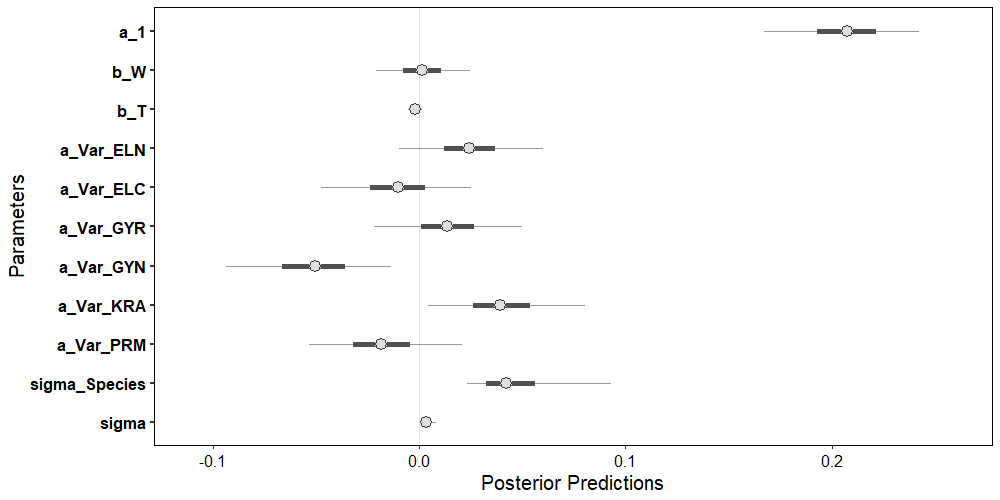
\includegraphics[width=\linewidth]{Params_Plot.png}
\caption{Posterior predictions for $M$ values as a function of log body mass and reconstructed temperature (model 1), showing maximum density posterior interval (dot), 50\% (thick line) and 90\% (thin line) highest density posterior intervals. ELN = \textit{Electrona antarctica}, ELC = \textit{E. carlsbergi}, GYR = \textit{Gymnoscopelus braueri}, GYN = \textit{G. nicholsi}, KRA = \textit{Krefftichthys anderssoni}, PRM = \textit{Protomyctophum bolini}.}
\label{fig:ParamsWT}
\end{figure}

Supplementary analyses (appendix \ref{app:supp}) % set appendix number
were unclear as to whether crushing whole otoliths, rather than milling, contributed to the lower \textdelta \textsuperscript{13}C in \textit{K. anderssoni}, and the resulting greater $M$ values for this species.

\subsection{$M$ Values with Temperature and Body Mass}

Posterior predictions of the scaling exponent of temperature for model 1 were negative ($b_{T}$ = -0.0020 \textpm 0.0022).
This suggests a slight negative linear relationship between $M$ values and reconstructed temperature (figures \ref{fig:ParamsWT} \& \ref{fig:WT}, and table \ref{tab:WT}).
There was no significant linear relationship between $M$ values and log body mass (figures \ref{fig:ParamsWT} \& \ref{fig:WT}, and table \ref{tab:WT}).

\clearpage
\begin{figure}[H]
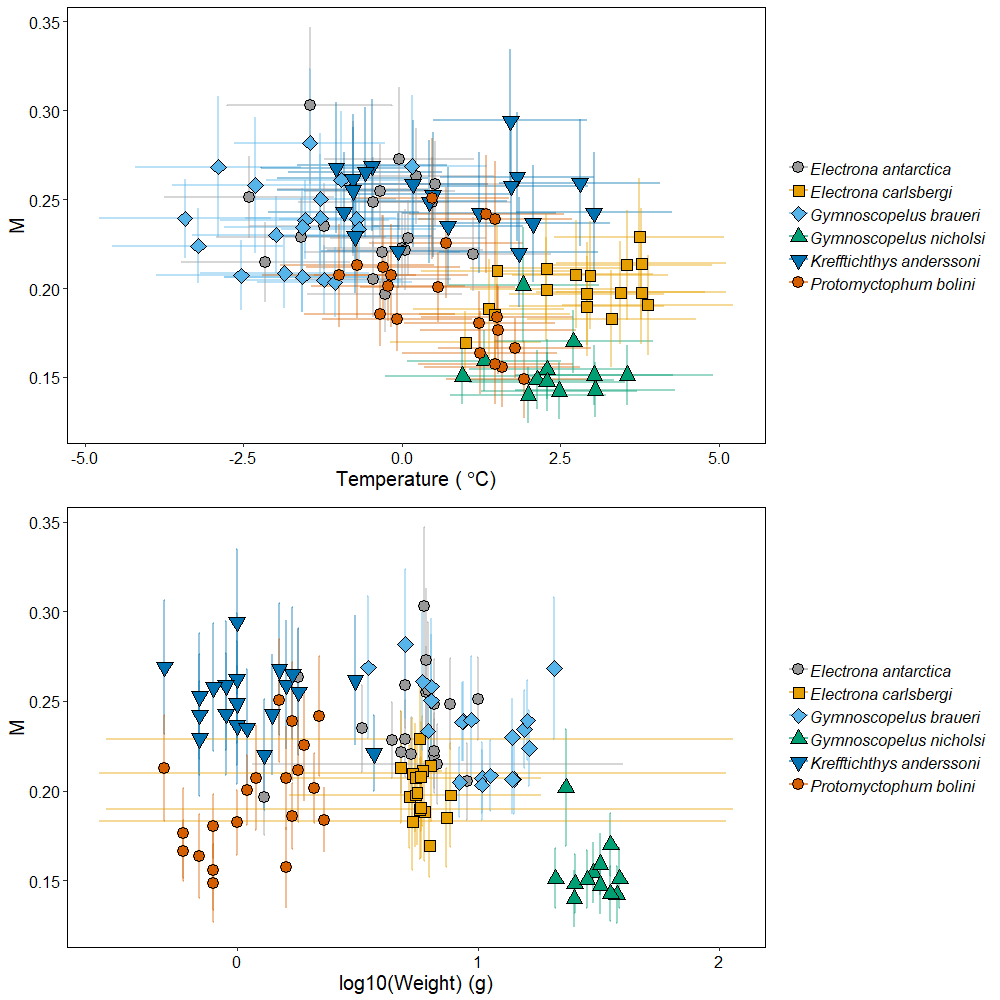
\includegraphics[width=\linewidth]{M_T_W.png}
\caption{Maximum density of distributions of $M$ values for individuals of six species of myctophids, with standard deviation bars, plotted against reconstructed temperature (\textdegree C) in the top graph and log body mass (g) in the bottom graph.}
\label{fig:WT}
\end{figure}

Within species, linear models of $M$ values and temperature (model 2) converged for all species except for \textit{E. carlsbergi} (table \ref{tab:SppT}.
In \textit{P. bolini}, the scaling exponent was significantly greater than zero (b = -0.0089 \textpm 0.0054), indicating that $M$ values decreased with increasing temperature in this species (figures \ref{fig:ParamsT} and \ref{fig:SppT}).

\begin{figure}[H]
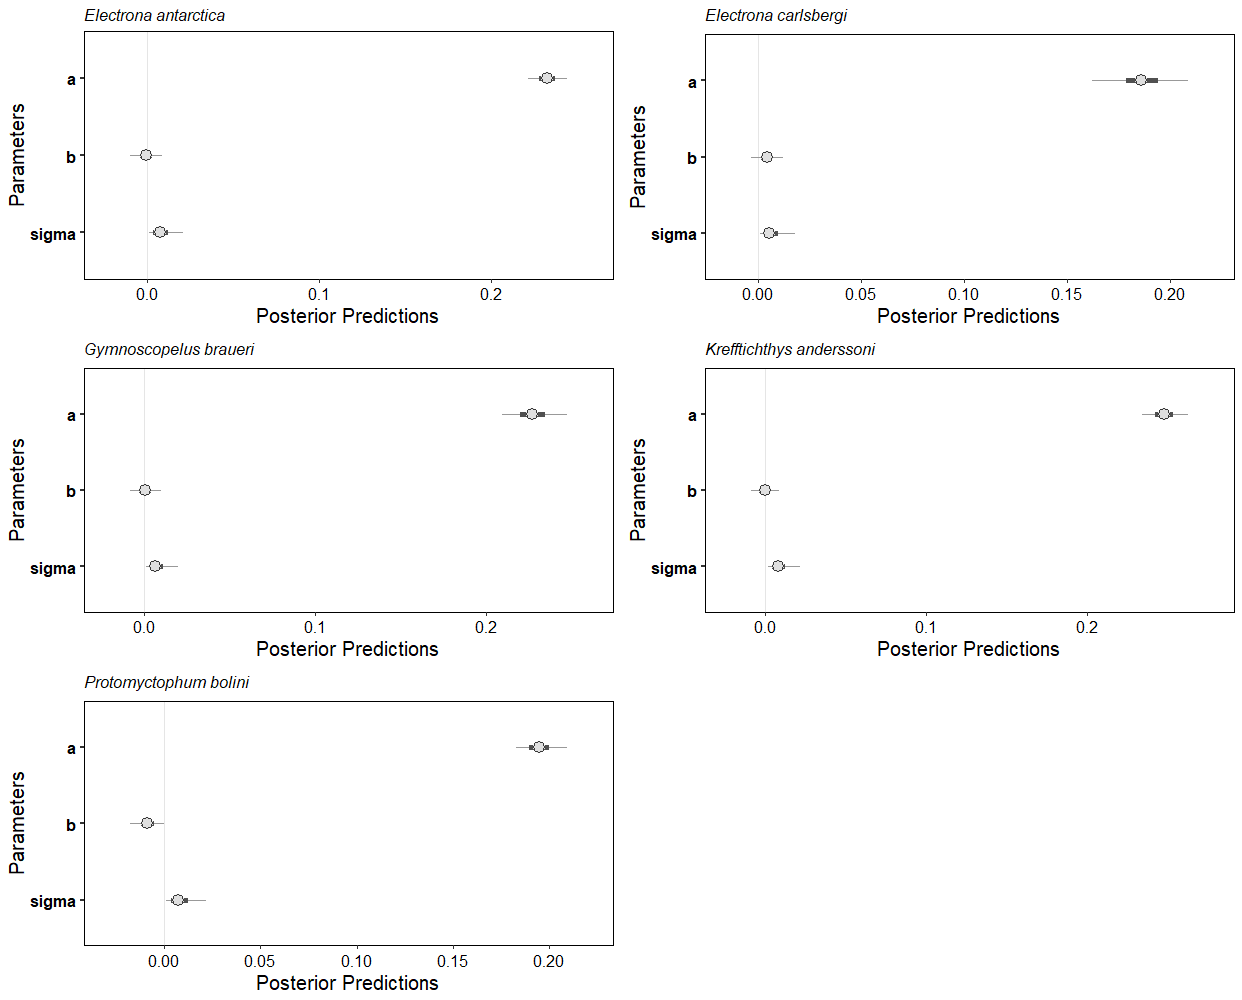
\includegraphics[width=\linewidth]{Params_Temp.png}
\caption{Posterior predictions for $M$ values as a function of reconstructed temperature, within species (model 2), showing maximum density posterior interval (dot), 50\% (thick line) and 90\% (thin line) highest density posterior intervals.}
\label{fig:ParamsT}
\end{figure}

\begin{table}[H]
\begin{center}
\caption{Posterior predictions of parameters from models of the relationship between temperature and $M$ values within species (model 2), with convergence and mixing diagnostics: number of effective samples (N\_eff) and \^R. ELN = \textit{Electrona antarctica}, ELC = \textit{E. carlsbergi}, GYR = \textit{Gymnoscopelus braueri}, GYN = \textit{G. nicholsi}, KRA = \textit{Krefftichthys anderssoni}, PRM = \textit{Protomyctophum bolini}.}
\label{tab:SppT}

\def\arraystretch{1.5}
  \begin{tabular}{ | l | l | l | l | l | l |}
    \hline
    \textbf{Species} & \textbf{Parameter} & Mean & SD & N\_eff & \^R \\ \hline
    \textbf{ELN} & a & 0.2196 & 0.0208 & 4334 & 1.00 \\ \hline
     & b & 0.0089 & 0.0122 & 4458 & 1.01 \\ \hline
     & $\sigma$ & 0.0099 & 0.0069 & 775 & 1.01 \\ \hline
     \textbf{ELC} & a & 0.2695 & 0.1087 & 45 & 1.06 \\ \hline
     & b & -0.0442 & 0.0601 & 43 & 1.06 \\ \hline
     & $\sigma$ & 0.0065 & 0.0084 & 5 & 1.31 \\ \hline
     \textbf{GYR} & a & 0.2275 & 0.0115 & 4489 & 1.00 \\ \hline
     & b & 0.0007 & 0.0057 & 3553 & 1.00 \\ \hline
     & $\sigma$ & 0.0081 & 0.0060 & 852 & 1.00 \\ \hline
     \textbf{GYN} & a & 0.1534 & 0.0133 & 6952 & 1.00 \\ \hline
     & b & -0.0007 & 0.0052 & 6654 & 1.00 \\ \hline
     & $\sigma$ & 0.0064 & 0.0049 & 1875 & 1.01 \\ \hline
     \textbf{KRA} & a & 0.2481 & 0.0086 & 8133 & 1.00 \\ \hline
     & b & -0.0004 & 0.0054 & 5378 & 1.00 \\ \hline
     & $\sigma$ & 0.0091 & 0.0065 & 1015 & 1.01 \\ \hline
     \textbf{PRM} & a & 0.1953 & 0.0080 & 3801 & 1.00 \\ \hline
     & b & -0.0089 & 0.0054 & 2922 & 1.00 \\ \hline
     & $\sigma$ & 0.0086 & 0.0066 & 889 & 1.00 \\
    \hline
  \end{tabular}
  \end{center}
\end{table}

\begin{figure}[H]
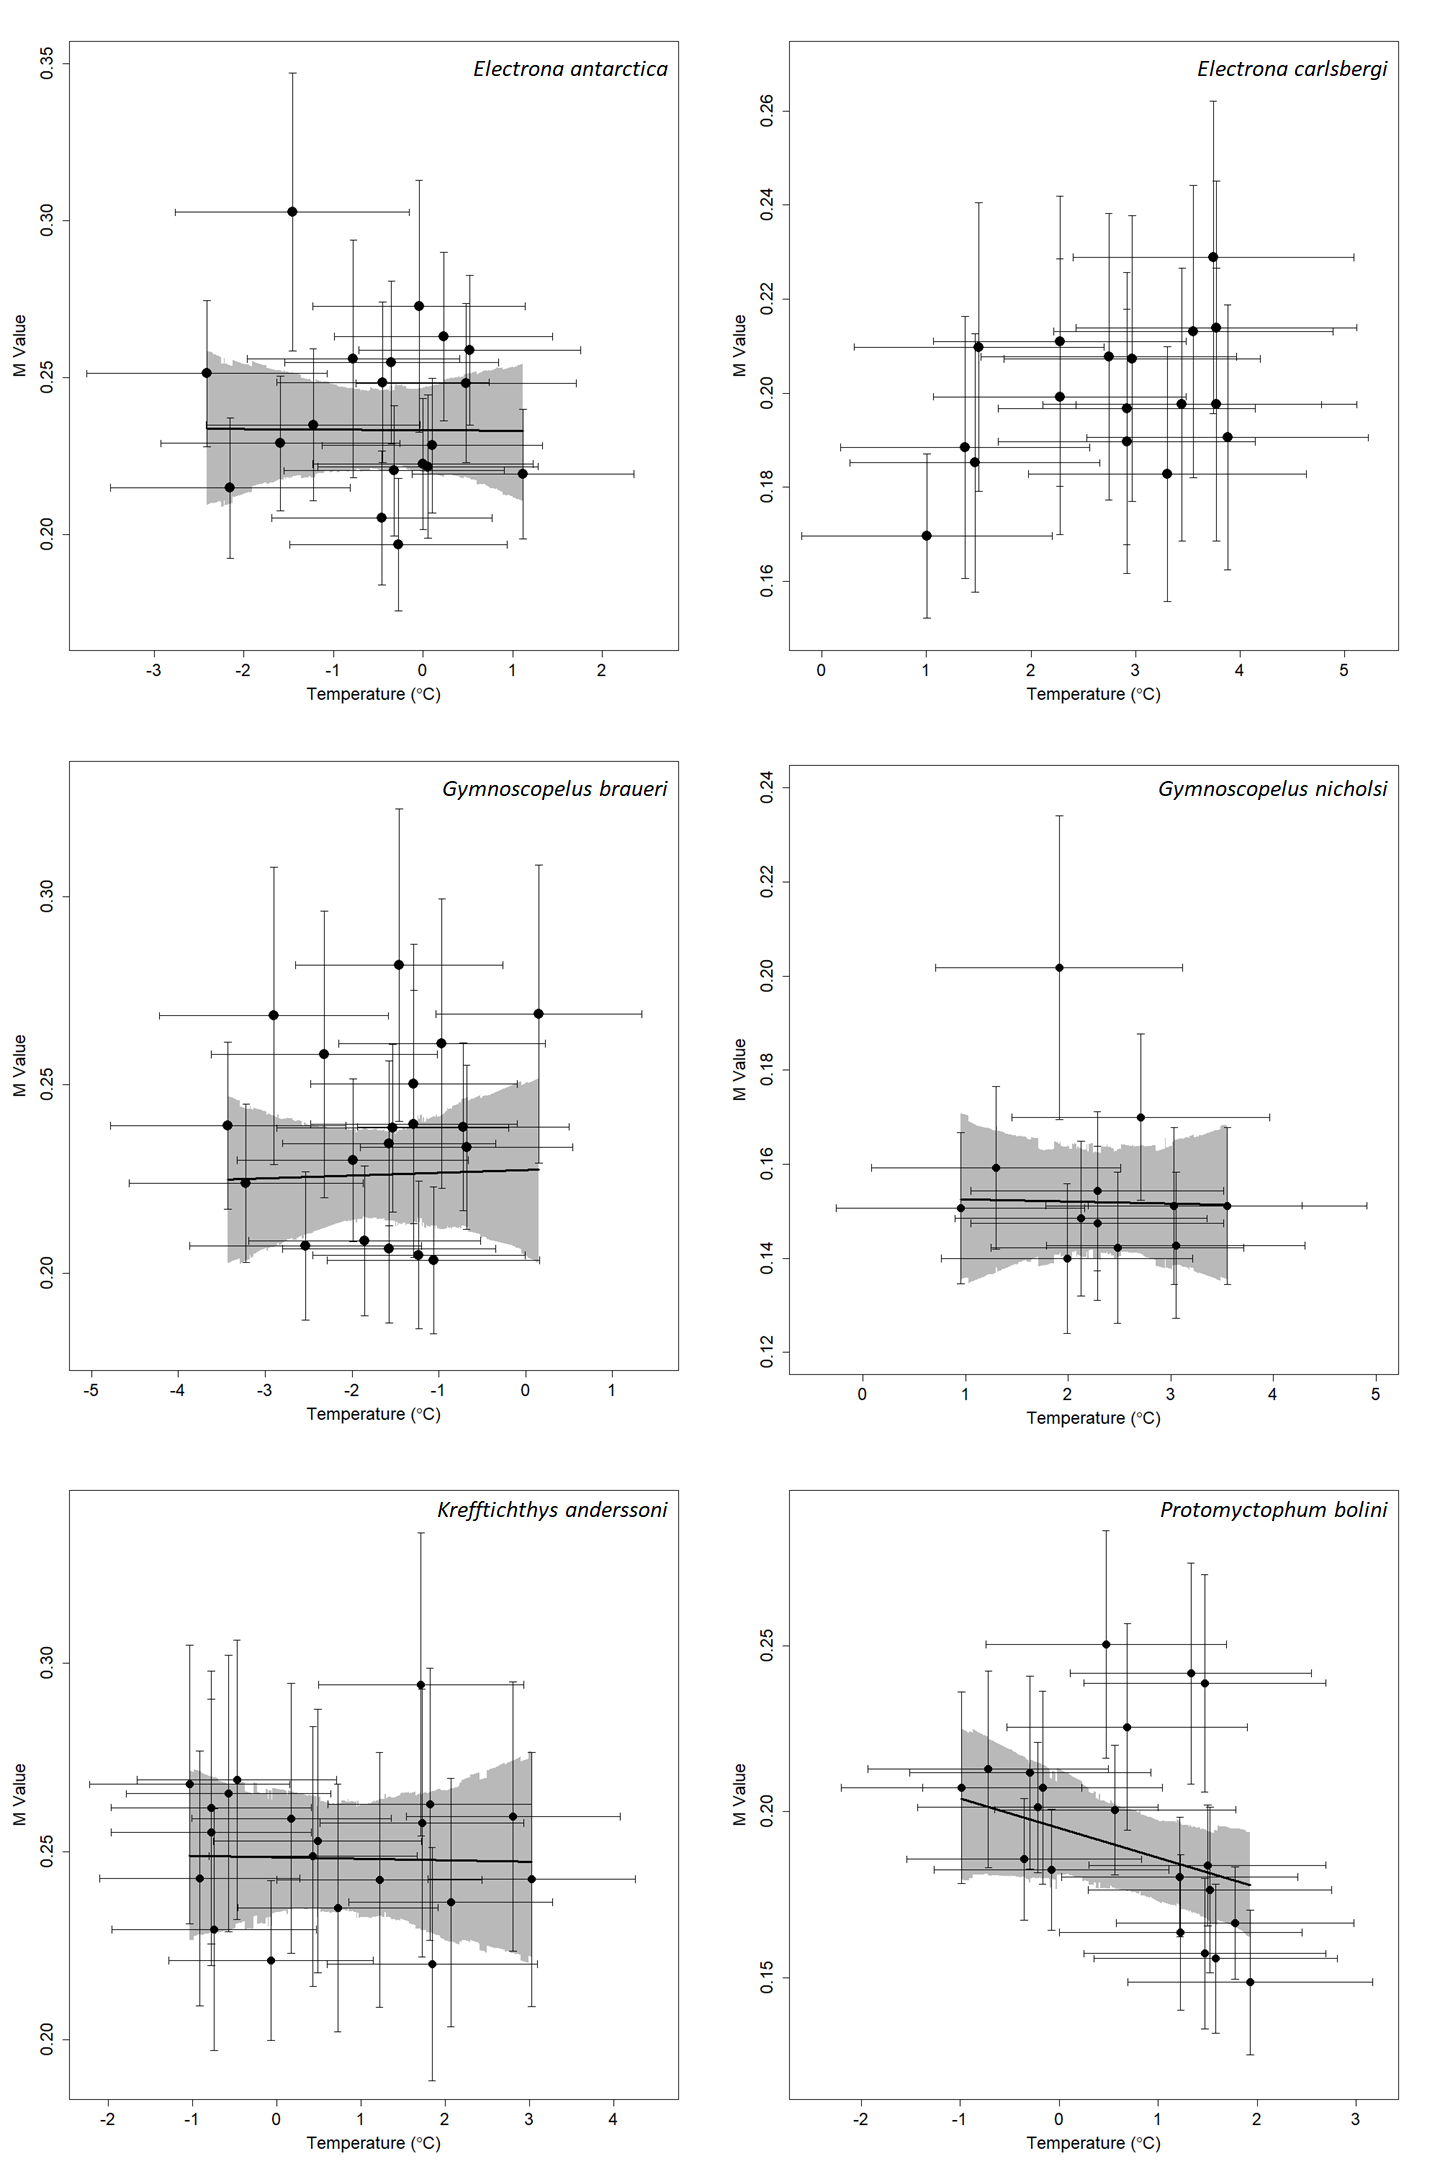
\includegraphics[width=\linewidth]{Combined_Temp.png}
\caption{Resonstructed temperature and $M$ values for each of the six species of myctophids. Where linear models converged (model 2), they are plotted with the means (solid line) and 95\% highest density posterior interval (shaded areas).}
\label{fig:SppT}
\end{figure}

Models of $M$ values with log body mass converged for \textit{E. antarctica, G. braueri} and \textit{P. bolini} (table \ref{tab:SppW}).
Models for the other three species did not converge (section \ref{sec:future}).

For \textit{E. antarctica} and \textit{G. braueri}, the scaling exponent was not significantly different from zero, suggesting that $M$ was invariant with log body mass in these species.
In \textit{P. bolini}, the scaling exponent was significantly greater than zero (b = 0.0257 \textpm 0.0118), indicating a that $M$ values increased with increasing log body mass (figures \ref{fig:ParamsW} and \ref{fig:SppW}).

\begin{figure}[H]
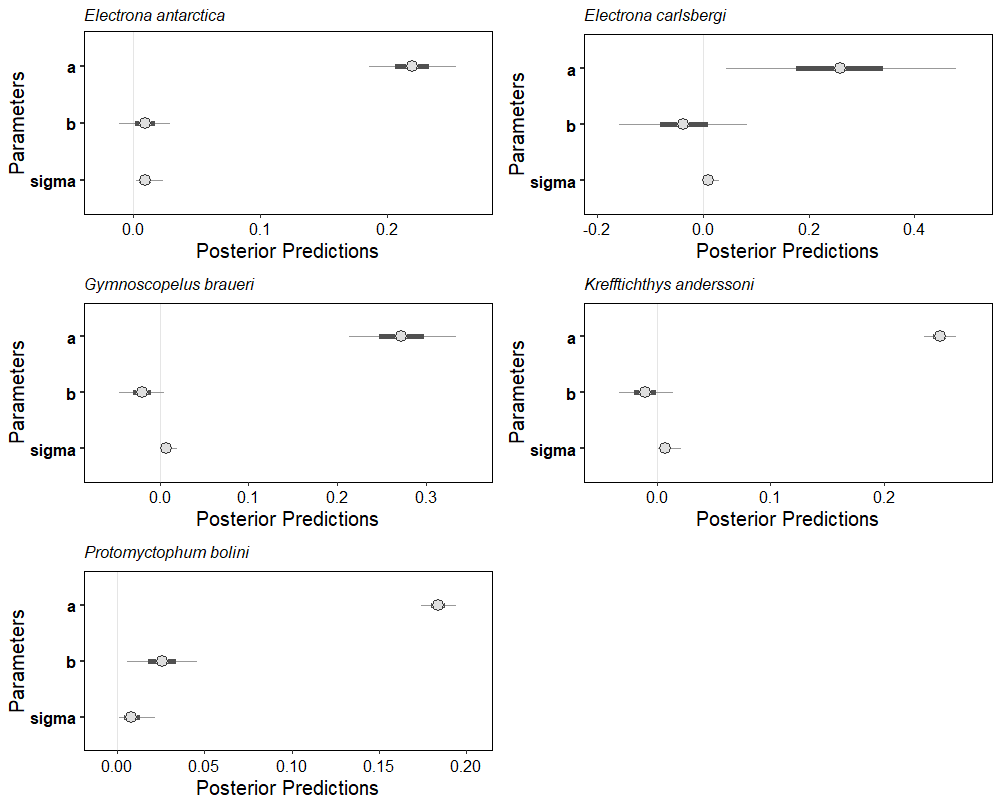
\includegraphics[width=\linewidth]{Params_Weight.png}
\caption{Posterior predictions for $M$ values as a function of log body mass, within species (model 3), showing maximum density posterior interval (dot), 50\% (thick line) and 90\% (thin line) highest density posterior intervals.}
\label{fig:ParamsW}
\end{figure}

\begin{table}[H]
\begin{center}
\caption{Posterior predictions of parameters from models of the relationship between log body mass and $M$ values within species (model 3), with convergence and mixing diagnostics: number of effective samples (N\_eff) and \^R. ELN = \textit{Electrona antarctica}, ELC = \textit{E. carlsbergi}, GYR = \textit{Gymnoscopelus braueri}, GYN = \textit{G. nicholsi}, KRA = \textit{Krefftichthys anderssoni}, PRM = \textit{Protomyctophum bolini}.}
\label{tab:SppW}

\def\arraystretch{1.5}
  \begin{tabular}{ | l | l | l | l | l | l |}
    \hline
    \textbf{Species} & \textbf{Parameter} & Mean & SD & N\_eff & \^R \\ \hline
    \textbf{ELN} & a & 0.2196 & 0.0210 & 7053 & 1.00 \\ \hline
    & b & 0.0090 & 0.0124 & 6692 & 1.00 \\ \hline
    & $\sigma$ & 0.0101 & 0.0069 & 1350 & 1.00 \\ \hline
    \textbf{ELC} & a & 0.2586 & 0.1328 & 4735 & 1.00 \\ \hline
    & b & -0.0365 & 0.0734 & 45731 & 1.00 \\ \hline
    & $\sigma$ & 0.0121 & 0.0096 & 285 & 1.01 \\ \hline
    \textbf{GYR} & a & 0.2720 & 0.0374 & 3454 & 1.00 \\ \hline
    & b & -0.0196 & 0.0156 & 3636 & 1.00 \\ \hline
    & $\sigma$ & 0.0086 & 0.0058 & 1203 & 1.01 \\ \hline
    \textbf{GYN} & a & 0.1836 & 0.0996 & 131 & 1.03 \\ \hline
    & b & -0.0095 & 0.0292 & 127 & 1.03 \\ \hline
    & $\sigma$ & 0.0062 & 0.0052 & 60 & 1.05 \\ \hline
    \textbf{KRA} & a & 0.2495 & 0.0087 & 2641 & 1.00 \\ \hline
    & b & -0.0101 & 0.0147 & 3538 & 1.00 \\ \hline
    & $\sigma$ & 0.0085 & 0.0065 & 765 & 1.01 \\ \hline
    \textbf{PRM} & a & 0.1840 & 0.0061 & 5421 & 1.00 \\ \hline
    & b & 0.0259 & 0.0122 & 6211 & 1.00 \\ \hline
    & $\sigma$ & 0.0094 & 0.0067 & 1174 & 1.00 \\
    \hline
  \end{tabular}
  \end{center}
\end{table}

\begin{figure}[H]
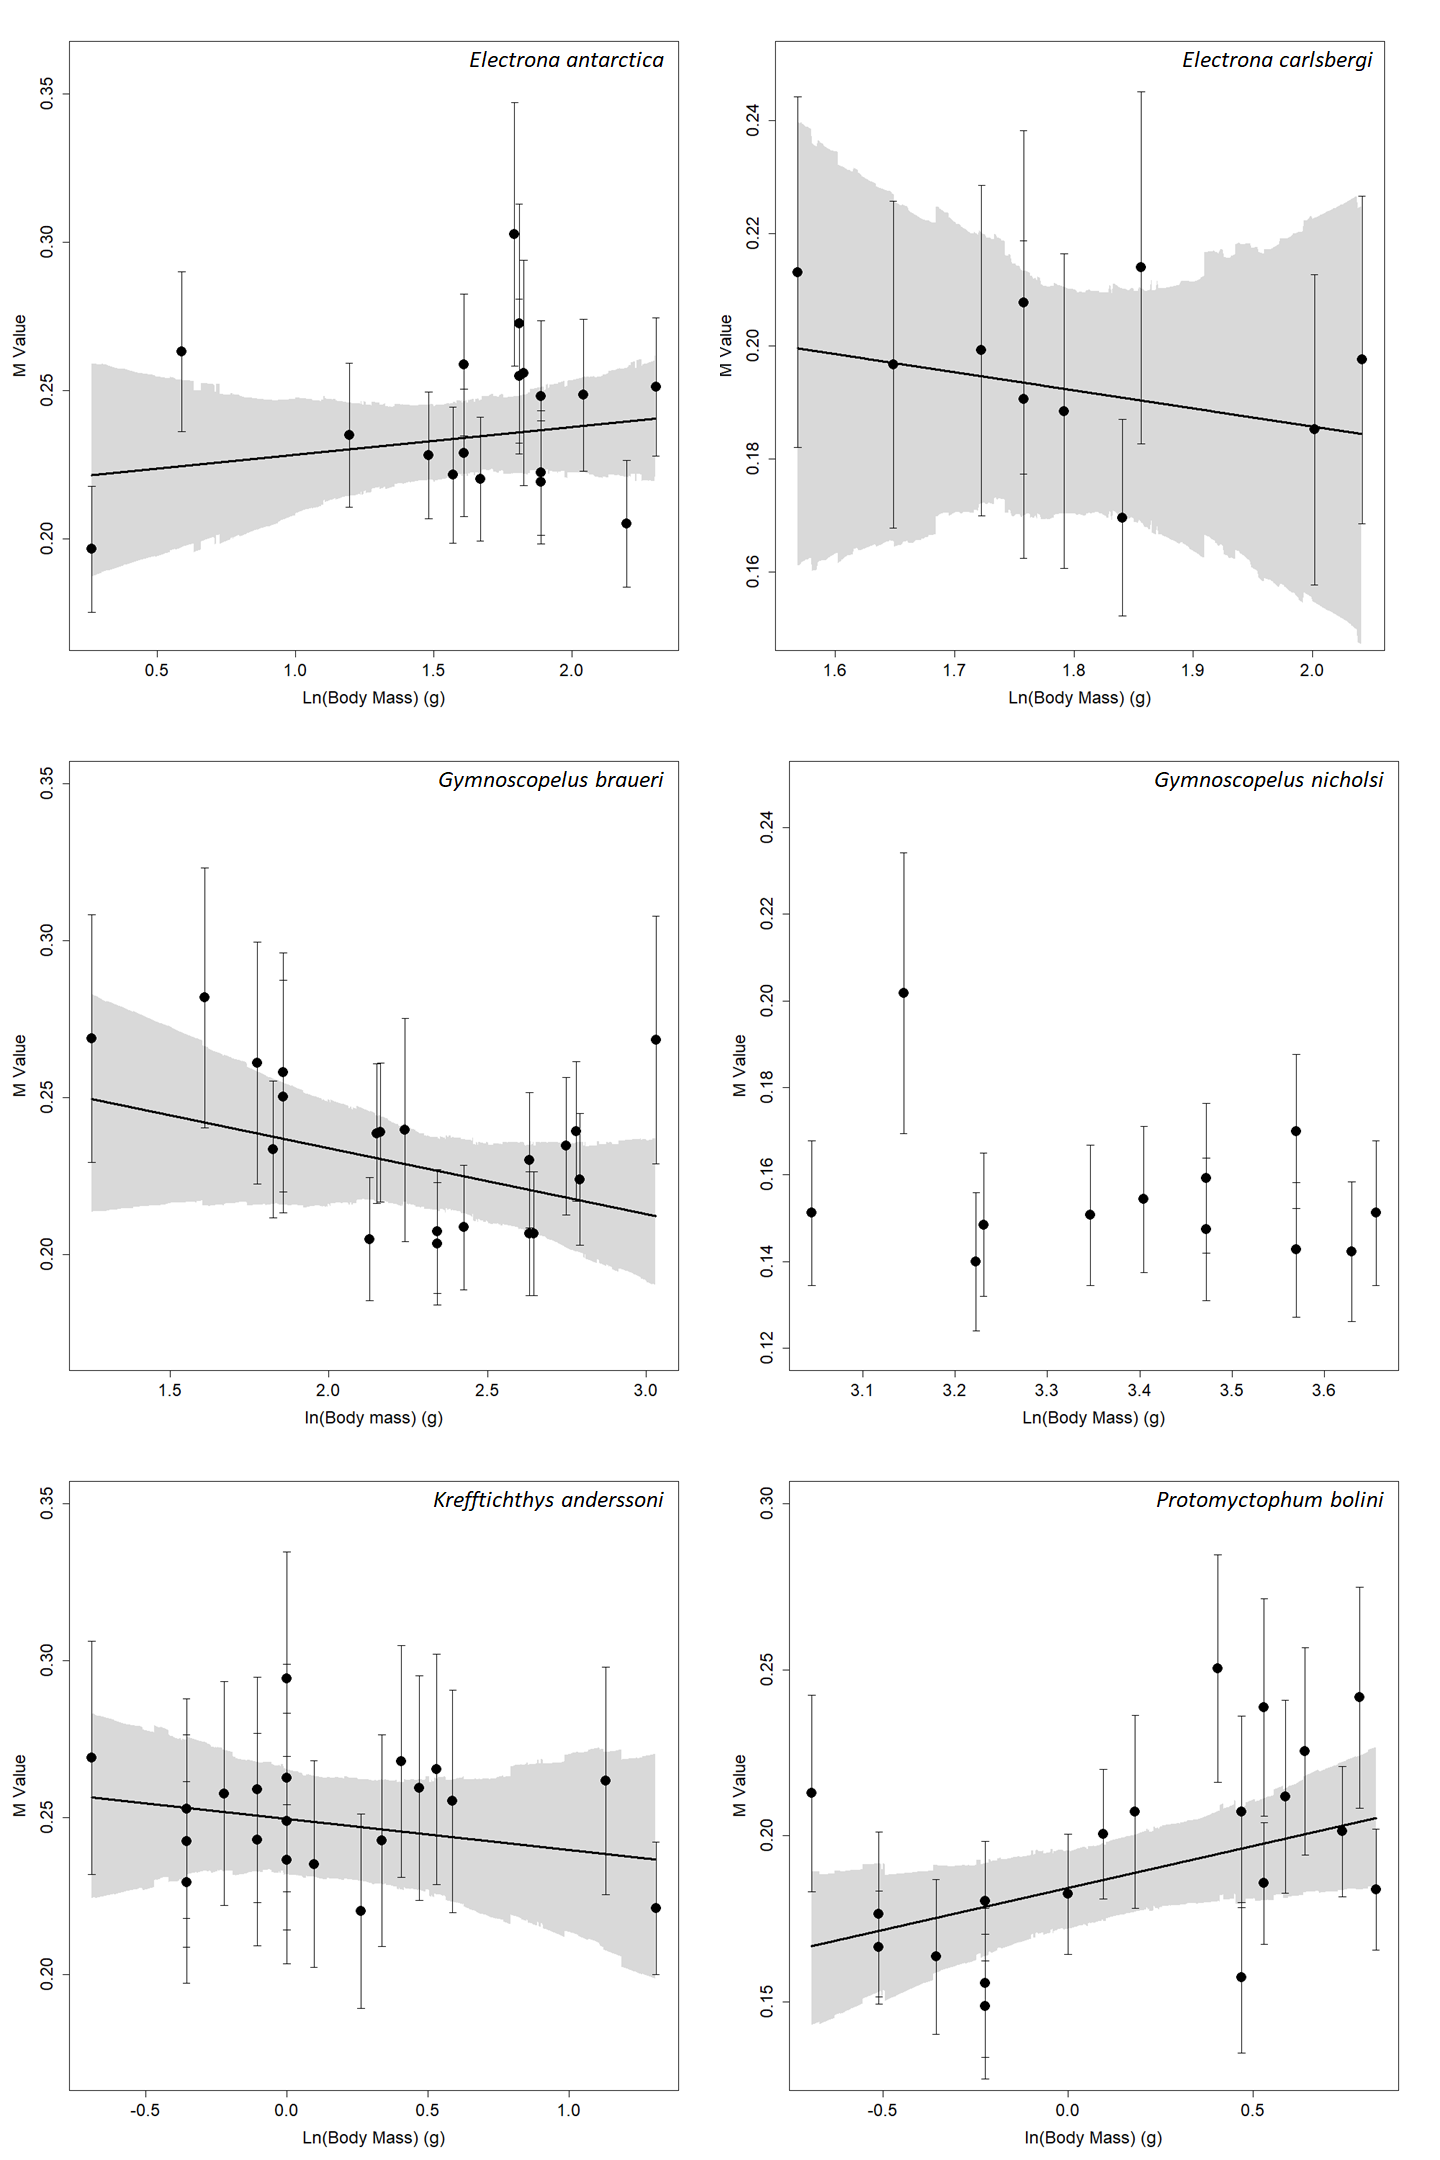
\includegraphics[width=\linewidth]{Combined_Weight.png}
\caption{Log body mass (g) and $M$ values for each of the six species. Where linear models (model 3) converged, they are plotted with the means (solid line) and 95\% highest density posterior interval (shaded areas).}
\label{fig:SppW}
\end{figure}

\subsection{Comparsion of Estimates of Metabolic Rate}

There was a significant negative correlation between estimates of log mass-specific RMR and $M$ values ($b$ = -0.0457 \textpm 0.0071) (figure \ref{fig:ParamsResp} and table \ref{tab:Resp}), therefore $M$ values decreased with increasing log mass-specific RMR (figure \ref{fig:Resp}).

\begin{figure}[H]
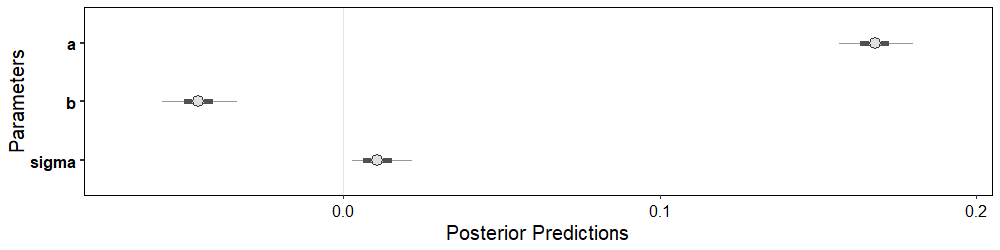
\includegraphics[width=\linewidth]{Params_Resp.png}
\caption{Posterior predictions for $M$ values and log mass-specific RMR (model 4), showing maximum density posterior interval (dot), 50\% (thick line) and 90\% (thin line) highest density posterior intervals. ELN = \textit{Electrona antarctica}, ELC = \textit{E. carlsbergi}, GYR = \textit{Gymnoscopelus braueri}, GYN = \textit{G. nicholsi}, KRA = \textit{Krefftichthys anderssoni}, PRM = \textit{Protomyctophum bolini}.}
\label{fig:ParamsResp}
\end{figure}

\begin{table}[H]
\begin{center}
\caption{Posterior predictions of parameters for $M$ values and log mass-specific RMR (model 4), with convergence and mixing diagnostics: number of effective samples (N\_eff) and \^R. ELN = \textit{Electrona antarctica}, ELC = \textit{E. carlsbergi}, GYR = \textit{Gymnoscopelus braueri}, GYN = \textit{G. nicholsi}, KRA = \textit{Krefftichthys anderssoni}, PRM = \textit{Protomyctophum bolini}.}
\label{tab:Resp}

\def\arraystretch{1.5}
  \begin{tabular}{ | l | l | l | l | l |}
    \hline
    \textbf{Parameter} & Mean & SD & N\_eff & \^R \\ \hline
    a & 0.1682 & 0.0072 & 901 & 1.01 \\ \hline
    b & -0.0457 & 0.0071 & 822 & 1.00 \\ \hline
    $\sigma$ & 0.0112 & 0.0059 & 244 & 1.01 \\
    \hline
  \end{tabular}
  \end{center}
\end{table}

\begin{figure}[H]
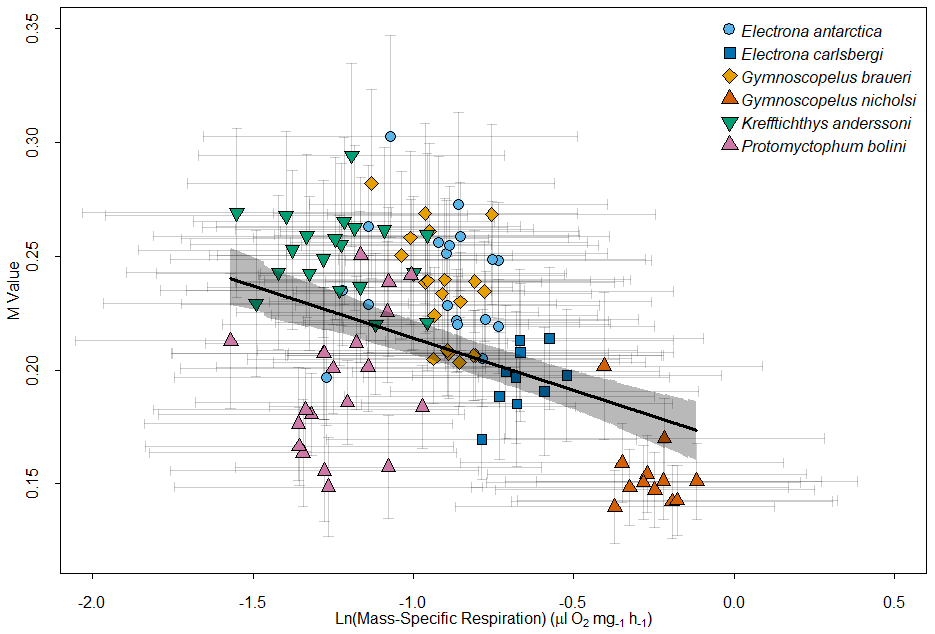
\includegraphics[width=\linewidth]{RMR_M.png}
\caption{Relationship between estimates of log mass-specific standard metabolic rate, derived from equation 1  and $M$ values, with standard deviation bars. Means (black line) and 95\% highest density posterior intervals (shaded) of posterior predictions from model 4 are overlayed.} 
\label{fig:Resp}
\end{figure}

\pagebreak
\section{Discussion}

\subsection{Species Differences in Relative Field Metabolic Rate}

This study showed that, despite overlap among them, species was the most useful variable in modelling $M$ values.
As temperature and body mass were accounted for, I theorise that this is due to differences in ecology among species.
Field metabolic rate (FMR) comprises of basal metabolic costs and energy for growth, reproduction, digestion, excretion and movement \citep{Treberg2016}.
While it is difficult to examine the other components of FMR, movement can be examined by comparing diel vertical migration strategies between species.

Different species of myctophids undertake diel vertical migration to different extents \citep{Watanabe1999, Catul2011}.
\textit{K. anderssoni, E. antarctica} and \textit{G. braueri} are all known to perform diel vertical migration year round  \citep{Torres1988b, Piatkowski1994, Collins2008, Saunders2015a, Lourenco2017}. 
These species also have a broad depth distribution, with individuals regularly found between 0-1000m depth \citep{GonHeemstra, Pusch2004, Saunders2014}.  
Individuals of these species are undertaking daily or near daily migrations across a large depth range, increasing the amount of respiration attributable to movement.
This may account for the larger mean $M$ values seen in these species.

In contrast, there is sparse evidence for diel vertical migration in \textit{G. nicholsi} or \textit{P. bolini} \citep{Saunders2015b, Collins2008},
and \textit{E. carlsbergi} undertakes diel vertical migration only in the summer \citep{Kozlov1991}.
Additionally, while individuals of these species are still occasionally found down to 1000m depth, the majority of the population stays above 700m in the case of \textit{G. nicholsi} \citep{Saunders2015a, Pusch2004, GonHeemstra}, % 2 7 10
 or above 400m for \textit{P. bolini} and \textit{E. carlsbergi} \citep{Saunders2014, Collins2012, Kozlov1991, Saunders2015b, Pusch2004}.
Given that these species are less likely to complete daily/near daily migrations, and if they do, are likely to be migrating across more compressed depth ranges, they are likely to have less respiration attributable to movement, which may explain their lower mean $M$ values.
Furthermore, there is evidence that \textit{G. nicholsi} individuals may become benthopelagic (living near the seafloor) during late adulthood \citep{Saunders2015a, GonHeemstra}.
This would reduce their movement compared to pelagic (living in the water column away from the seafloor) fishes, resulting in a lower FMR, and could explain why this species had significantly lower$M$ values than the other five species.

\subsection{Temperature and Body Mass}

There was a slight negative relationship between temperature and $M$ values, which may be an artefact of differing ecological factors between species.
Species with the lowest mean $M$ values (\textit{G. nicholsi}, \textit{P. bolini} and \textit{E. carlsbergi}) are more common in the north of the Scotia Sea, where water temperatures are warmer. \citep{Collins2012, Saunders2014, Piatkowski1994, GonHeemstra, Saunders2015b}. 
There is also evidence that these species do not complete their life cycles within the Scotia Sea, as the temperatures are too low for the more sensitive larval stages.
Recruitment for these species may occur outside of the Scotia Sea, with adults migrating in from elsewhere \citep{Saunders2015a, Saunders2014, Collins2012, Collins2008}.
This would mean that these species are living at the lowest end of their thermal range, which may inhibit their metabolic rates \citep{Clarke1999, Killen2010, Portner2008}.

In contrast, species with the highest mean $M$ values (\textit{K. anderssoni, E. antarctica} and \textit{G. braueri}) are more common in the colder, more southerly waters of the Scotia Sea.
These species are truly Antarctic, with all life stages found in the Scotia Sea \citep{Saunders2014, GonHeemstra, Saunders2015a, Lourenco2017, Collins2012, Collins2008}.
Individuals of these species are more likely to be living well within their thermal range, and therefore able to maintain higher metabolic rates, explaining the higher $M$ values  \citep{Clarke1999, Killen2010, Portner2008}.
More research on otoliths from individuals of \textit{G. nicholsi}, \textit{P. bolini} and \textit{E. carlsbergi} from sites north of the Scotia Sea would be needed to to confirm this theory. 
However, given that temperature was not significantly correlated with $M$ values within most species, and that species captured the most variation in $M$ values, it seems likely that any negative correlation between species is an artefact.

Within species, log body mass and temperature were only significantly correlated with $M$ values in \textit{P. bolini}.
Within \textit{P. bolini}, $M$ values increased with increasing log body mass, and decreased with increasing temperature.
This is the opposite of what would be expected according to metabolic theory, and relationships of $M$ values with log body mass and temperature in previous studies, where mass-specific metabolic rate, and therefore $M$ values, decreased with increasing body mass, and increased with increasing temperature \citep{Portner2008, Killen2010, Clarke1999, Brown2004, Trueman2016}.
The reason for this is unclear, and more measurements of $M$ values in this species, across a range of body masses, would be needed to investigate this further.

\subsection {Resting and Field Metabolic Rate}

The negative linear relationship of $M$ values and log mass-specific resting metabolic rate (RMR) suggests that fishes with a high RMR have a low FMR, contrary to previous studies and metabolic theories \citep{Brown2004, Killen2016}.
If we assume that equation 1 generates reasonable estimates for values of log mass-specific RMR, this suggests that the other components of FMR (thermic effect of food, growth, reproduction, movement and excretion) have a larger influence on FMR than RMR does.
These factors are more likely to be influenced by ecological differences among species, and this is supported by the result that species had the greatest influence on $M$ values.

There are issues with how the equation was parameterised which may affect any inferences drawn from it.
Two of the studies used to parameterise equation 1 gave mass-specific RMR based on electron transport system activity (ETS) \citep{Belcher2019}.
ETS is converted to mass-specific RMR using ratios which varied between the two studies.
For example, one study used an ETS/RMR ratio of 2,\citep{Ariza2015}
while another used a ratio of 1.16 \citep{Ikeda1989}.
The ETS/RMR ratio of 2 was used based on a study of zooplankton, \citep{herna1996factors}
while the ETS/RMR ratio of 1.16 was based the author's results from gobies (family Gobiidae) and pomacentrids (family Pomacentridae).
Uncertainty around the ETS/RMR ratio was not accounted for when calculating log mass-specific RMR from ETS, and consequently was not incorporated when parameterising equation 1.
Studies used to parameterise equation 1 had a much greater temperature range (0.5 to 20 \textdegree C) than was estimated for the fishes in our study (-3.4 to 3.9 \textdegree C, maximum density posterior values).
This may have overinflated the postive relationship between metabolic rate and temperature when comparing fishes from the relatively narrow range of temperatures in the Scotia Sea.

Variation in $M$ values, and therefore FMR, is not adequately captured using log body mass, temperature or estimated log RMR as predictors.
Given this, and the discussed issues in parameterisation, equation 1 is not adequate enough in accurately predicting metabolic rate to be used in carbon modelling.
Ecological factors such as migratory strategy are likely to be better predictors of FMR, but more research is needed across a wider range of species to confirm which ecological factors have the most influence on FMR.

\pagebreak
\section{Future Work}
\label{sec:future}

This work will become one of the chapters of my thesis, and the first paper from my PhD project.
When rewriting, I will make two main changes.

First, sensitivity analysis for $M$ values across a range of species (appendix \ref{app:Sens}) indicated that $\delta^{13}C_{phytoplankton}$, which is used to estiamte $\delta^{13}C_{diet}$ had the greatest influence on the maximum density of $M$. 
The \textdelta \textsuperscript{13}C value of muscle tissue, corrected for trophic fractionation factor, is a reasonable approximation of the $\delta^{13}C_{diet}$ of an individual fish \citep{DeNiro1978}.
Each otolith used in this study also came with muscle tissue, which has been analysed for \textdelta \textsuperscript{13}C.
Unfortunately, these data were not available when this report was in preparation.
However, for the thesis chapter and paper manuscript, $M$ values will be recalculated using this data, ensuring a more accurate and precise estimate for each fish.
I will also work on putting the $M$ and temperature functions into a Bayesian framework.

Many Hamiltonian Monte Carlo (HMC) simulations in this study did not converge.
In future analyses, for my thesis chapter and when this is written into a paper, I will run HMC with a single, long chain, as opposed to four short chains, as was done with model 1.
I will also re-examine the priors and thinning parameters used in this model.

\pagebreak
\section{Thesis Plan and Gantt Chart}

\subsection{Overview of PhD}

The broad aim of my PhD is to investigate how the field metabolic rate (FMR) of fishes varies at a macroecological scale. 
The work in this report forms the basis for chapter four of my PhD thesis and a research paper.
Target journals for this paper are Marine Ecology Progress Series, Journal of Fish Biology or Polar Biology.

Aside from this and an introduction (chapter one), I plan on three other chapters, outlined here.
Each chapter, apart from the introduction, will be written up into a paper.

\subsection{Chapter 2: $M$ Values Dataset}
\label{sec:Data}

The first step of my PhD has been to build up a dataset of $M$ values from otolith isotope \textdelta \textsuperscript{13}C from a range of species of fishes across a range of ecological categories and taxonomy.
The dataset currently consists of 42 species, with otoliths from a further 25 species awaiting stable isotope analysis.
Each species is represented by otoliths from ten individuals, and must have associated catch location and year, and a measure of body size.
The majority of the stable isotope analysis will take place in late 2019, when I visit the Life Sciences Mass Spectrometry Facility (figure \ref{fig:Gantt}).
The dataset presently has good representation across benthopelagic (fishes living near seafloor) and deep-sea fishes, but is lacking in pelagic (fishes living in the water column away from the seafloor) and migratory fishes.
I am working on filling this gap by forming collaborations with other otolith researchers, and collecting otoliths from the Split fish market in Croatia.
Once other papers are published, we will publish this dataset as a data paper, to make it available to the wider scientific community.
Target journals for this paper are Ecology, PLOS One or Ecological Research.

\subsection{Chapter 3: Body Mass and Temperature Scaling}

There are several theories as to how metabolic rate scales with body mass and temperature, and how it varies between species, including the metabolic theory of ecology \citep{Brown2004} and the metabolic level boundaries hypothesis \citep{Glazier2005}.
These theories are used to predict how species might respond to climate change, and were initially developed using basal metabolic rate (BMR) data from endotherms, analogous to standard or resting metabolic rate (RMR) in ectotherms.
As discussed in the above report, FMR is the more appropriate measure of metabolic rate in a modelling context.

There have been no studies examining how body mass and temperature scale with FMR in fishes. 
The common method for studying FMR in endotherms, the doubly-labelled water technique does not work in fishes, due to their high water turnover rates \citep{Treberg2016}.
The otolith isotope technique for $M$ values, is ideal for investigating FMR at a macroecological scale, as otoliths archives are numerous, primarly due to their use in ageing fishes \citep{Campana1998}.
I will use phylogenetic comparative methods to account for phylogenetic non-independence; the principle that species are not independent data points, due to their shared evolutionary history \citep{Harvey1991}.
Target journals for this paper are Ecology Letters, Biology Letters or Journal of Animal Ecology.

\subsection{Chapter 5: Ecological Influences on $M$ Values}

From reading previous macroecological studies of fish metabolic rate, I am interested in which ecological factors significantly influence $M$ values, and therefore FMR.
Ecological factors I will examine are habitat (benthic, benthopelagic or pelagic), \citep{Killen2010, Killen2016}
depth, \citep{Drazen2007, Seibel2007, Killen2010, Killen2016}
body shape, \citep{Uyeda2017, Sherwood2003}
migratory habits and schooling or shoaling behaviours.
I will also investigate whether $M$ values correlated with growth, as estimated through the $k$ term in the von Bertalanffy growth equation.
As with chapter three, I will use phylogenetic comparitive methods in my analysis.
I will also compare $M$ values across the fish phylogenetic tree.
This chapter and paper may split into several, depending on the results of the analyses.
Target journals for this paper are Proceedings of the Royal Society B, Ecology and Evolution or Marine Ecology Progress Series.

\pagebreak
\begin{landscape}
\subsection{Gantt Chart}

\begin{figure}[H]
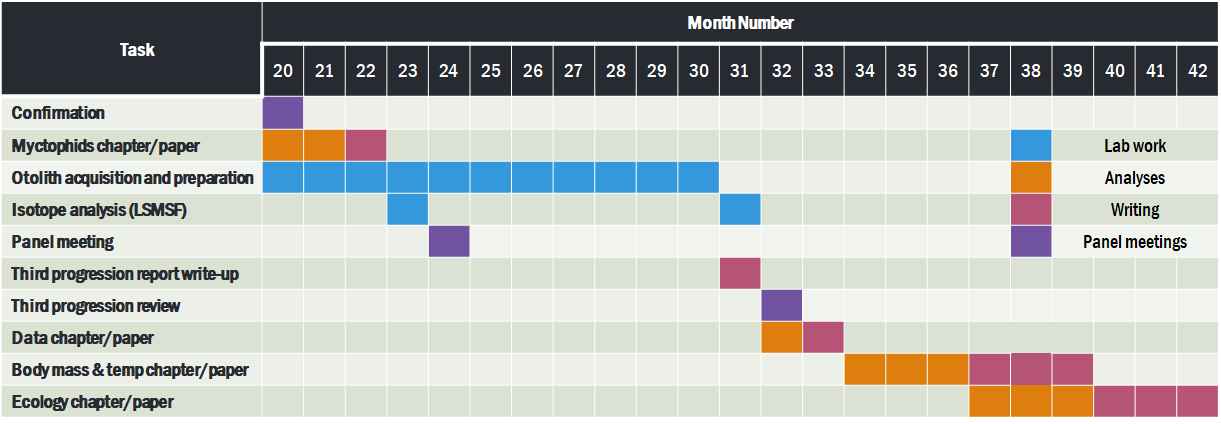
\includegraphics[width=\linewidth]{Gantt.png}
\caption{Gantt chart of expected progress until the end of my PhD.}
\label{fig:Gantt}
\end{figure}

\end{landscape}

\pagebreak
\section{Acknowledgements}

Thank you to Dr. Gabriele Stowasser and the British Antarctic Survey for donating the otoliths used in this study.
Special thanks to my supervisors Dr. Clive Trueman, Dr. Natalie Cooper and Mr. Oliver Crimmen for their ongoing support with all my research, and for providing constructive feedback on earlier versons of this report.
Assistance in mounting the otoliths provided by Mr. Joseph Jones, Mr. Daniel Doran and Mr. Matthew Beverley-Smith is greatly appreciated.
Thank you also to Mr. Bastian Hambach and Mrs. Megan Wilding for running the stable isotope analyses.
This work is supported by the Natural Enviornment Research Council [grant number NE/L002531/1].

\pagebreak
\bibliography{Refs}
\bibliographystyle{plainnat}

\pagebreak
\appendix

\includepdf[pages=1,pagecommand={\section{$M$ Values Function}, \thispagestyle{empty}}, fitpaper=true]{C:/Users/sra2g13/Documents/PhD/GitHub/mytophid-ears/Confirmation/Appendices/PseudoBayes_M.pdf}
\includepdf[pages=2-,pagecommand={\thispagestyle{empty}}, fitpaper=true]{C:/Users/sra2g13/Documents/PhD/GitHub/mytophid-ears/Confirmation/Appendices/PseudoBayes_M.pdf}

\includepdf[pages=1,pagecommand={\section{Temperature Function}, \thispagestyle{empty}}, fitpaper=true]{C:/Users/sra2g13/Documents/PhD/GitHub/mytophid-ears/Confirmation/Appendices/PseudoBayes_Temp.pdf}
\includepdf[pages=2-,pagecommand={\thispagestyle{empty}}, fitpaper=true]{C:/Users/sra2g13/Documents/PhD/GitHub/mytophid-ears/Confirmation/Appendices/PseudoBayes_Temp.pdf}


\section{Supplementary Analyses}
\label{app:supp}

There was no significant difference between maximum density estimates of $M$ values between otolith samples that were milled and crushed (F(1, 18) = 1.63, p = 0.218) in \textit{Protomyctophum bolini}, the only species for which otoliths were both crushed and milled.
Across all species, with species as a random factor, maximum density estimates of $M$ values were slightly lower for milled compared to crushed otoliths (estimate of effect of milling = -0.03112 \textpm 0.01519).

\section{Traceplots}

\subsection{Model 1 - Body Mass and Temperature}
\begin{figure}[H]
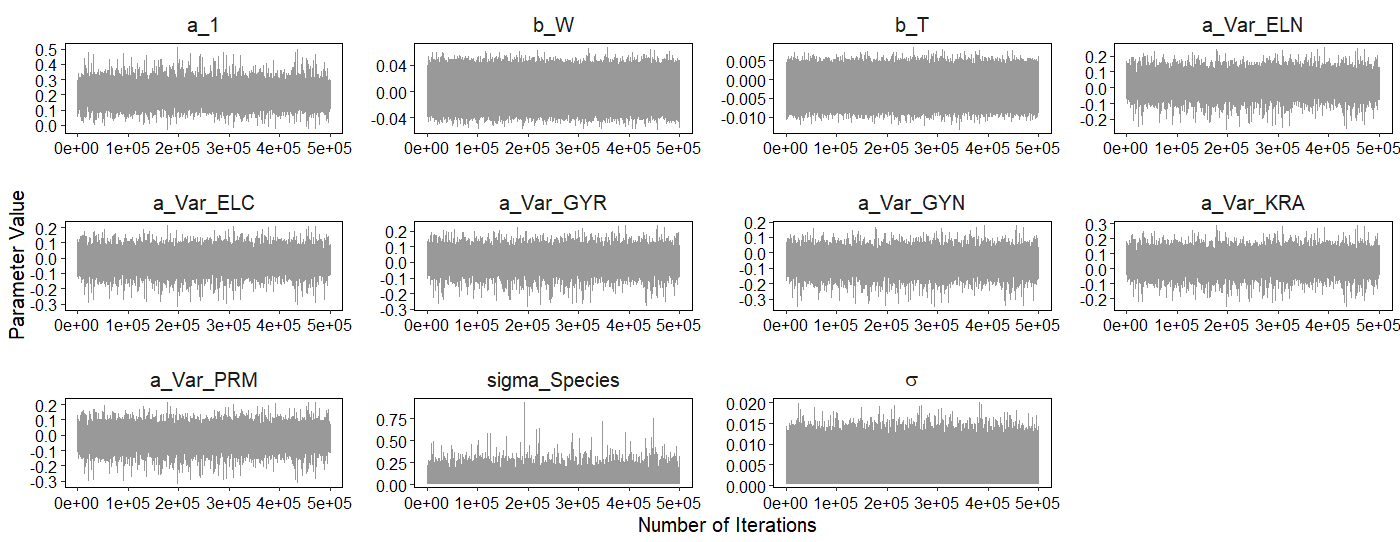
\includegraphics[width=\linewidth]{Traceplot_W_T.png}
\end{figure}

\subsection{Model 2 - Temperature}
\begin{figure}[H]
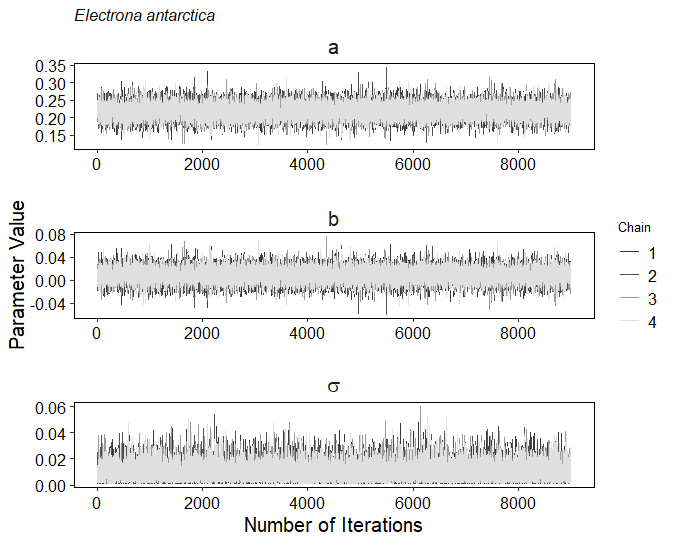
\includegraphics[width=\linewidth]{Traceplot_ELN_T.png}
\end{figure}
\begin{figure}[H]
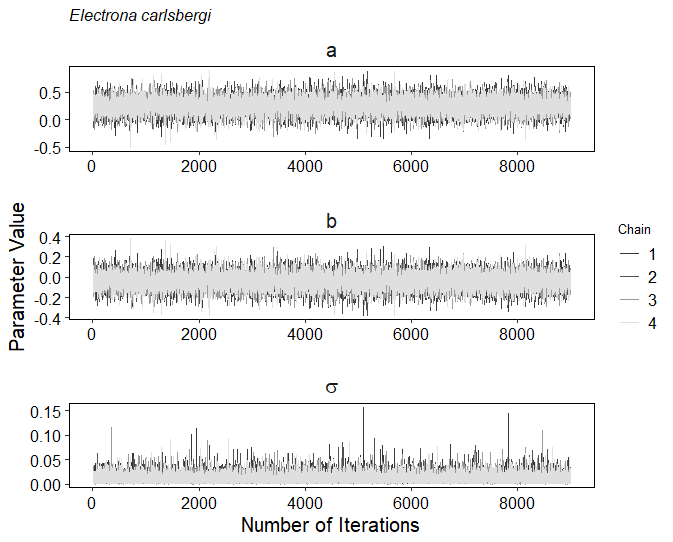
\includegraphics[width=\linewidth]{Traceplot_ELC_T.png}
\end{figure}
\begin{figure}[H]
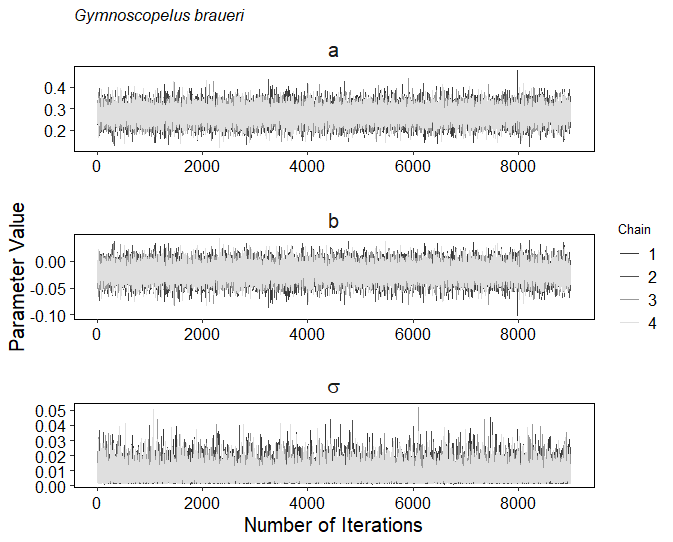
\includegraphics[width=\linewidth]{Traceplot_GYR_T.png}
\end{figure}
\begin{figure}[H]
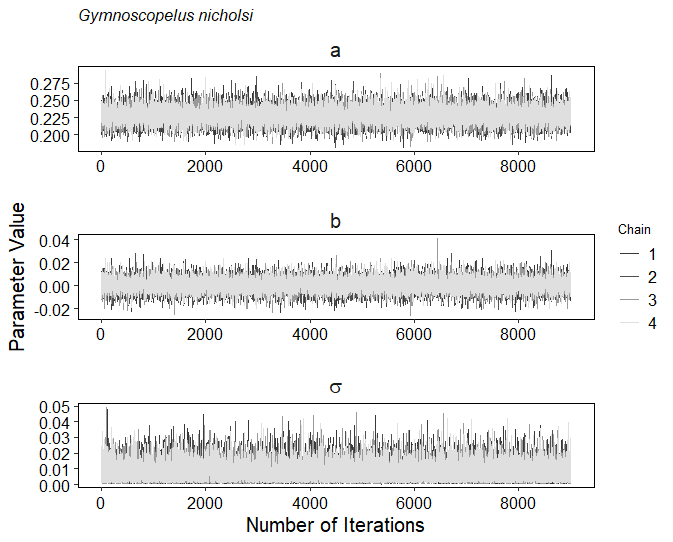
\includegraphics[width=\linewidth]{Traceplot_GYN_T.png}
\end{figure}
\begin{figure}[H]
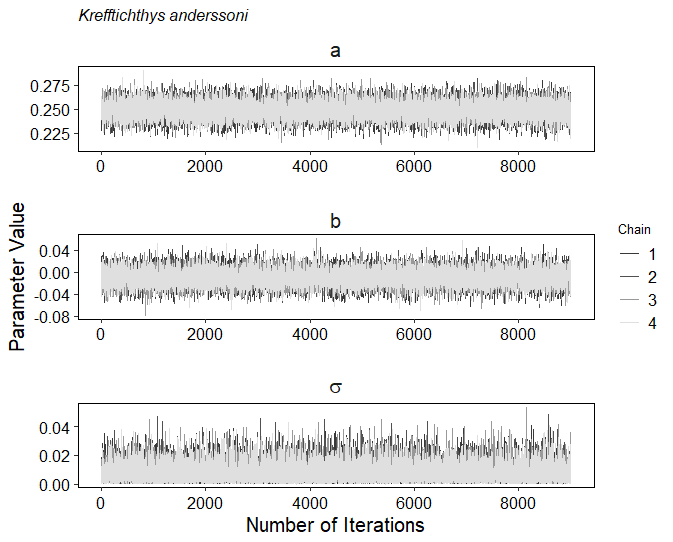
\includegraphics[width=\linewidth]{Traceplot_KRA_T.png}
\end{figure}
\begin{figure}[H]
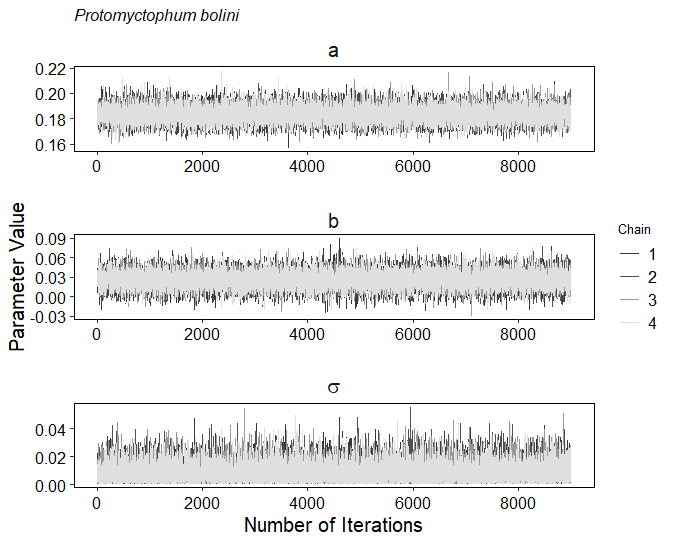
\includegraphics[width=\linewidth]{Traceplot_PRM_T.png}
\end{figure}

\subsection{Model 3 - Body Mass}

\begin{figure}[H]
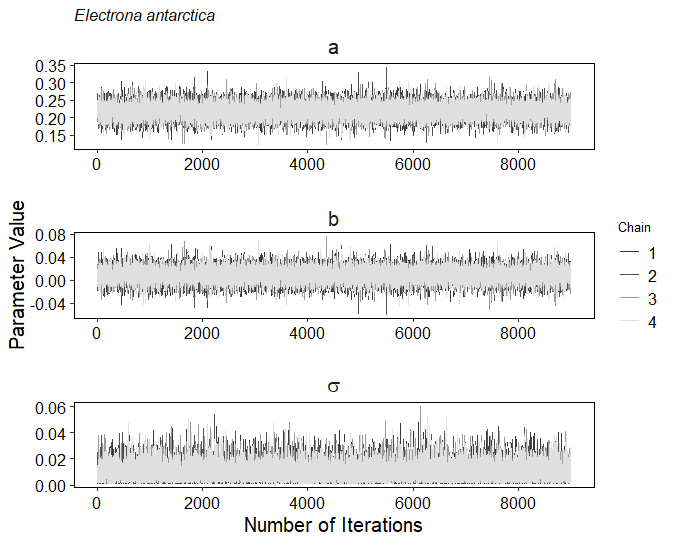
\includegraphics[width=\linewidth]{Traceplot_ELN_W.png}
\end{figure}
\begin{figure}[H]
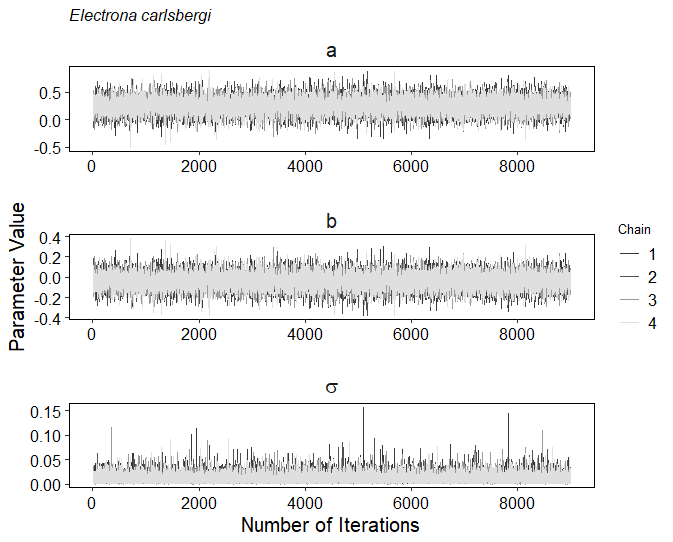
\includegraphics[width=\linewidth]{Traceplot_ELC_W.png}
\end{figure}
\begin{figure}[H]
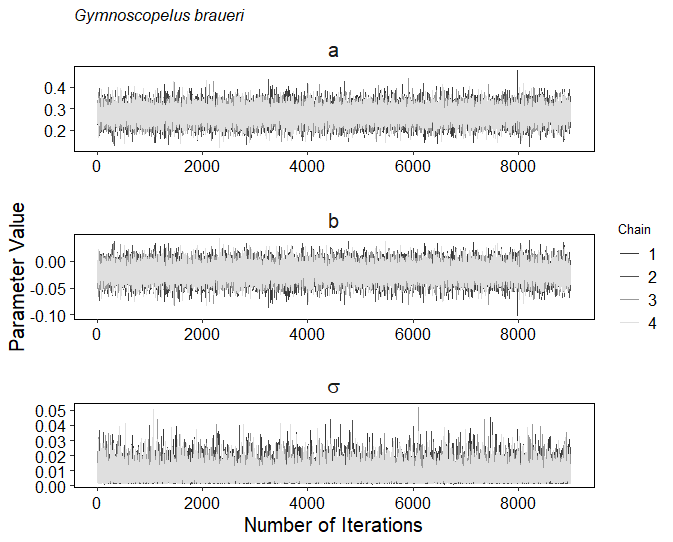
\includegraphics[width=\linewidth]{Traceplot_GYR_W.png}
\end{figure}
\begin{figure}[H]
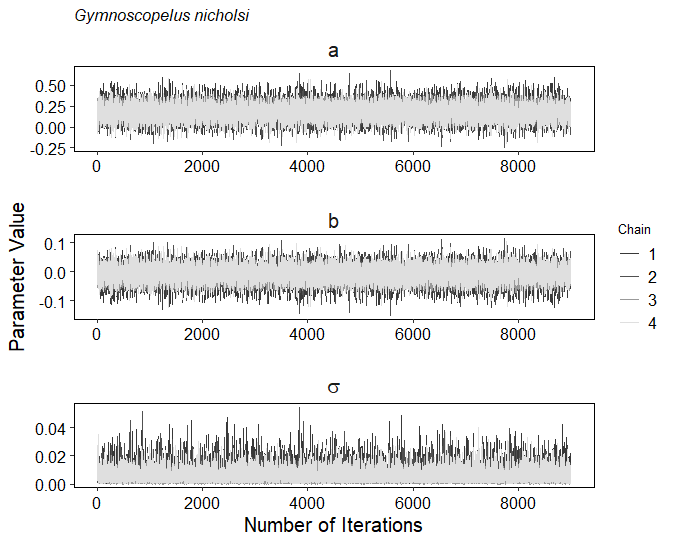
\includegraphics[width=\linewidth]{Traceplot_GYN_W.png}
\end{figure}
\begin{figure}[H]
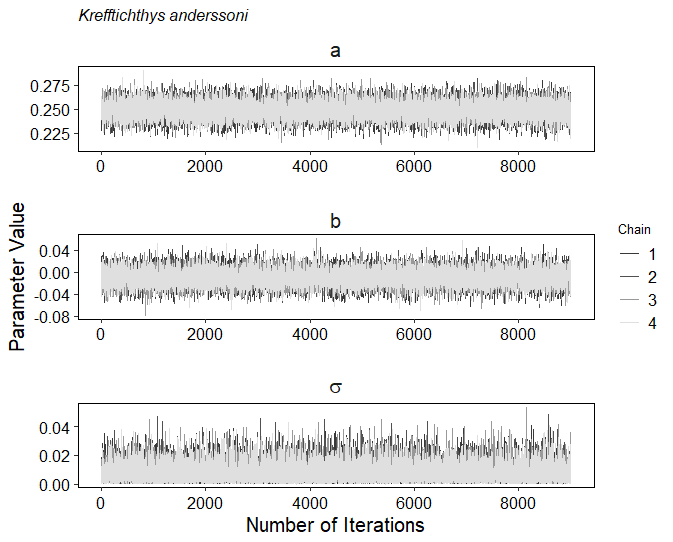
\includegraphics[width=\linewidth]{Traceplot_KRA_W.png}
\end{figure}
\begin{figure}[H]
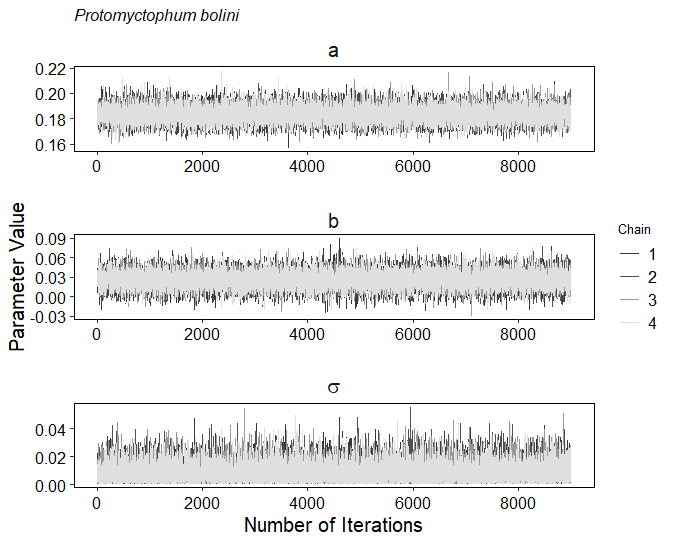
\includegraphics[width=\linewidth]{Traceplot_PRM_W.png}
\end{figure}


\subsection{Model 4 - Resting Metabolic Rate}
\begin{figure}[H]
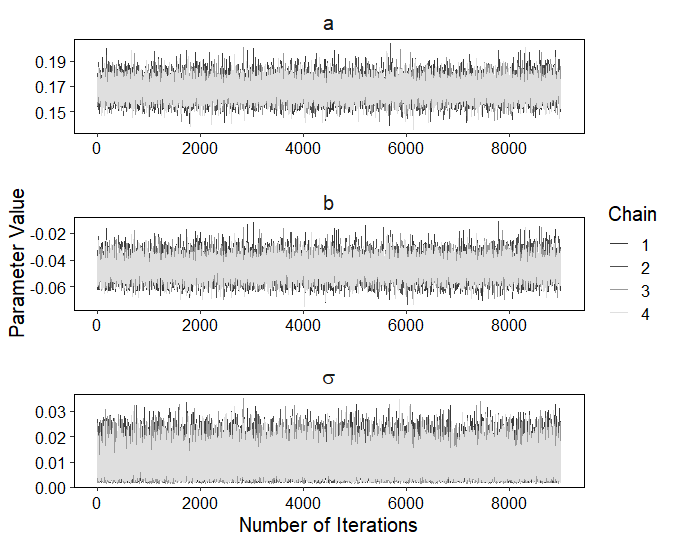
\includegraphics[width=\linewidth]{Traceplot_Resp.png}
\end{figure}

\pagebreak
\section{Sensitivity Analysis for $M$ Function}
\label{app:Sens}

This sensitivity analysis was carried out on my main data set (section \ref{sec:Data}).
The violin plots show the distribution of maximum density of $M$ values for individuals from this dataset.
Violins marked ``baseline'' have values set according to those used in this study (section \ref{sec:M}).

\begin{figure}[H]
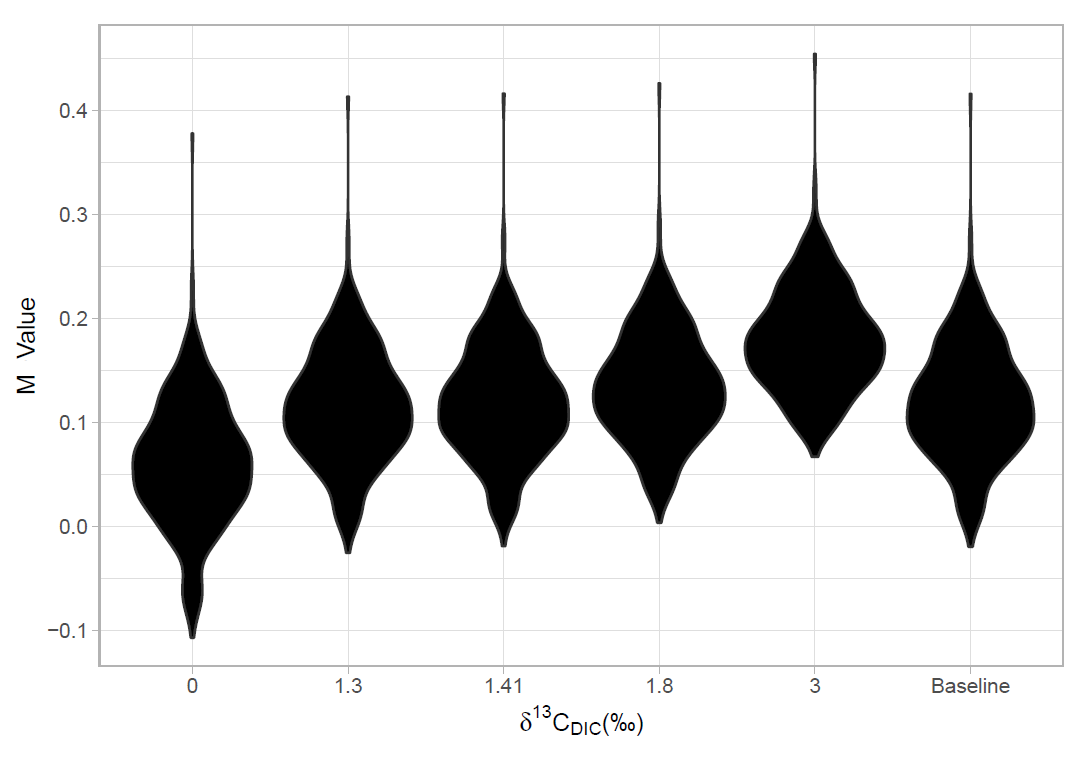
\includegraphics[width=\linewidth]{Sens_DIC.png}
\end{figure}

\begin{figure}[H]
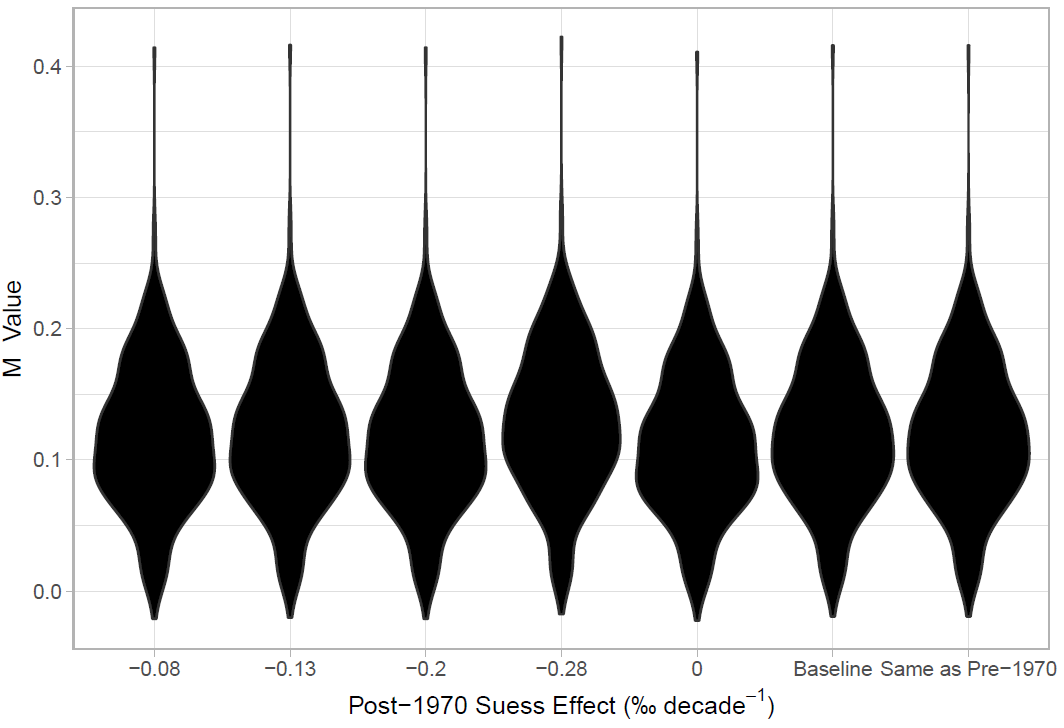
\includegraphics[width=\linewidth]{Suess.png}
\end{figure}

\begin{figure}[H]
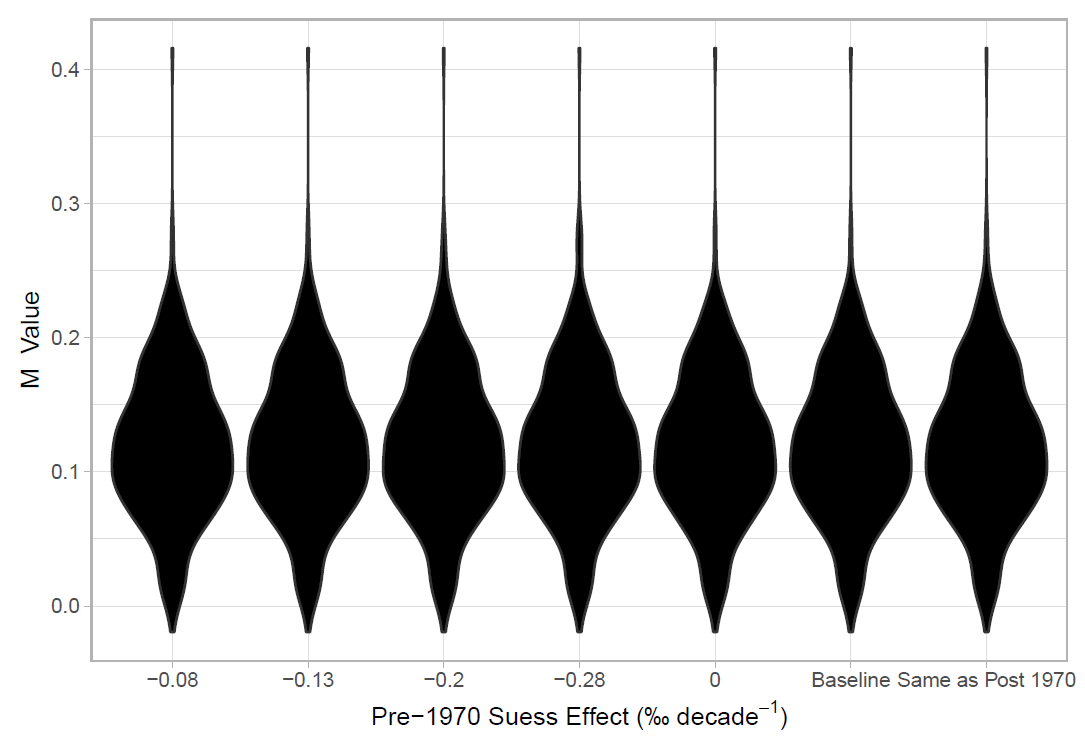
\includegraphics[width=\linewidth]{Suess_1970.png}
\end{figure}

\begin{figure}[H]
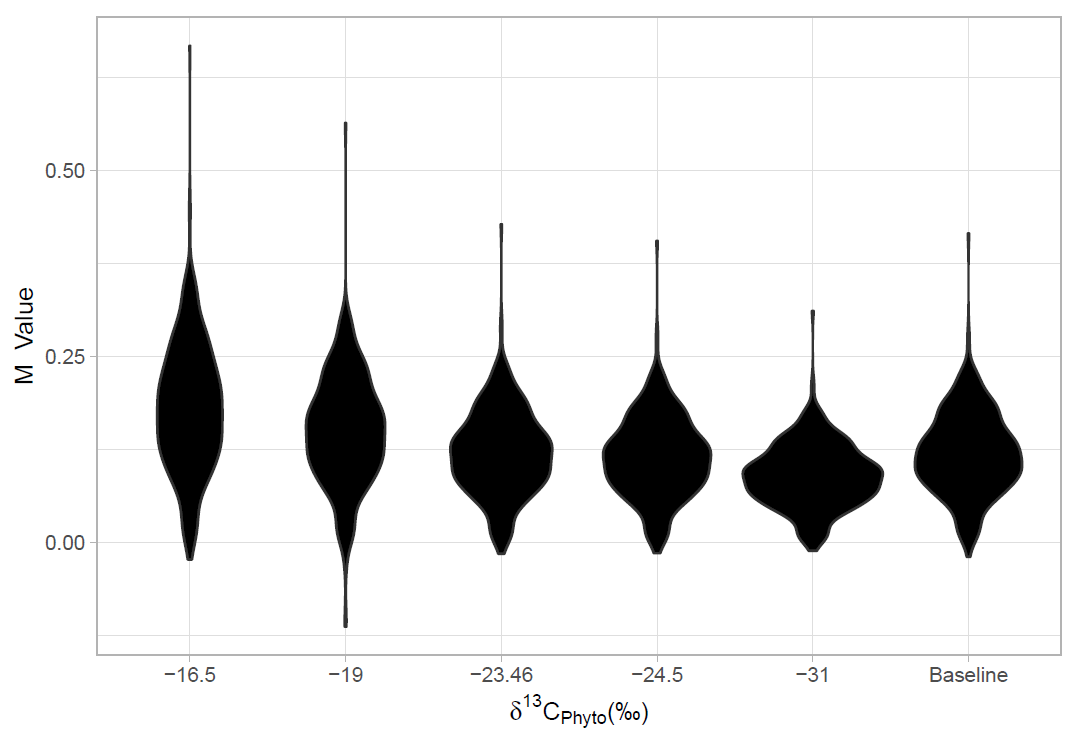
\includegraphics[width=\linewidth]{Sens_Phyto.png}
\end{figure}

\begin{figure}[H]
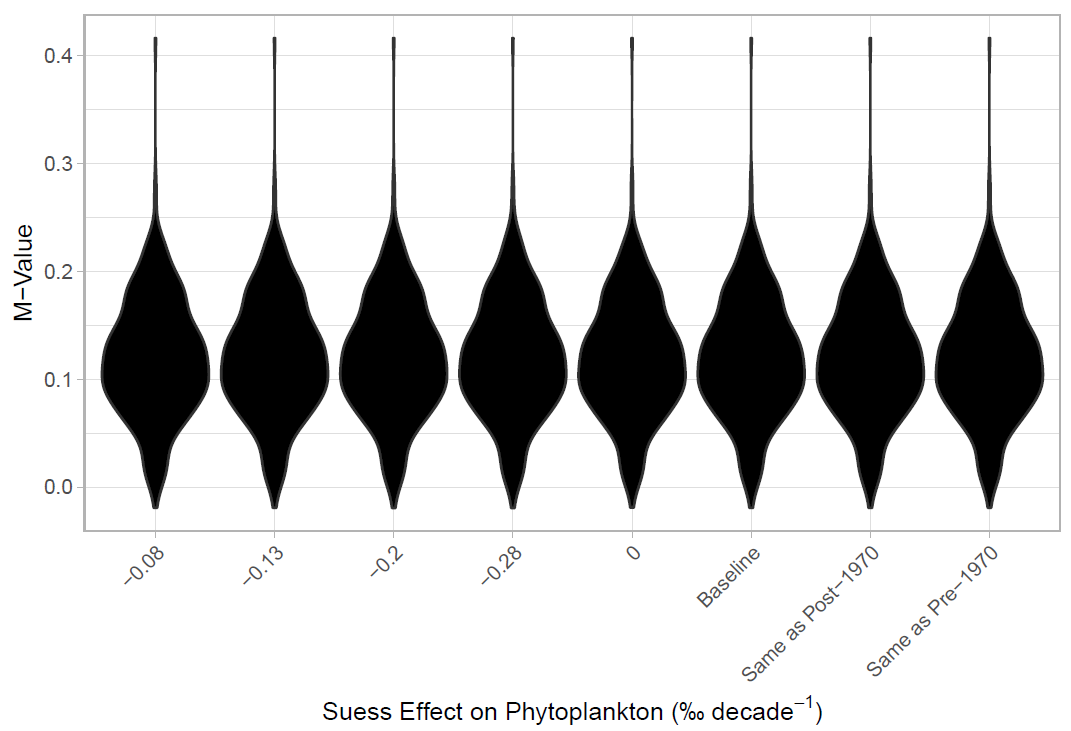
\includegraphics[width=\linewidth]{Suess_Phyto.png}
\end{figure}

\begin{figure}[H]
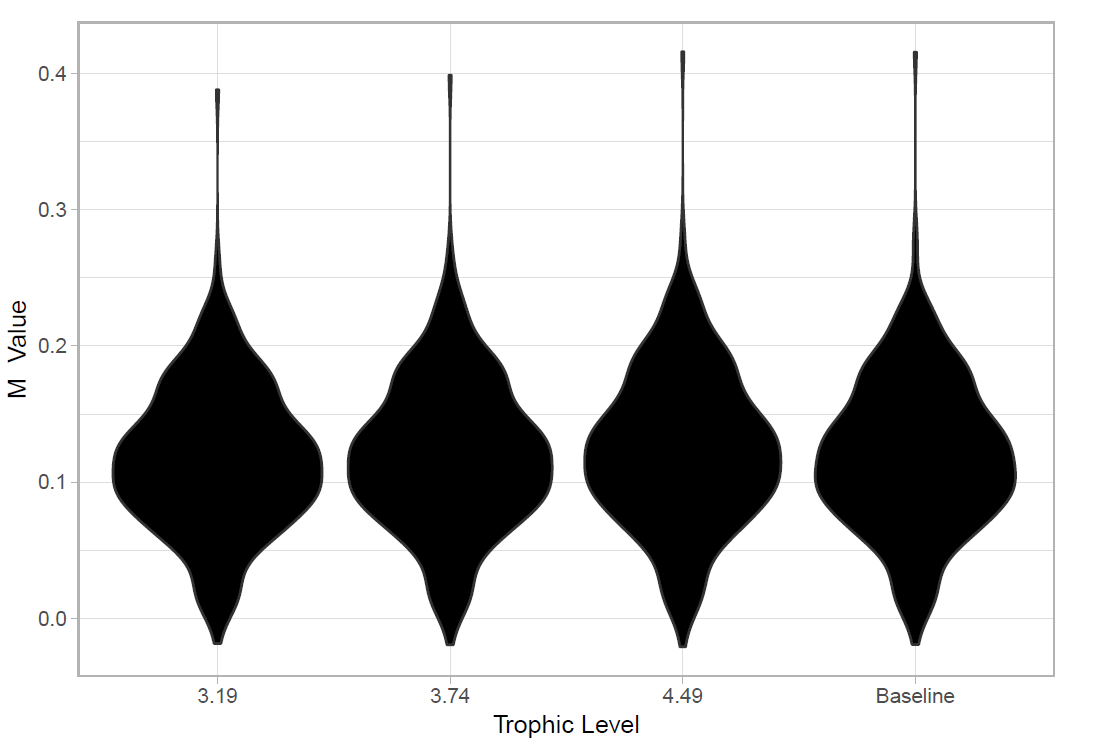
\includegraphics[width=\linewidth]{Sens_Troph.png}
\end{figure}

\begin{figure}[H]
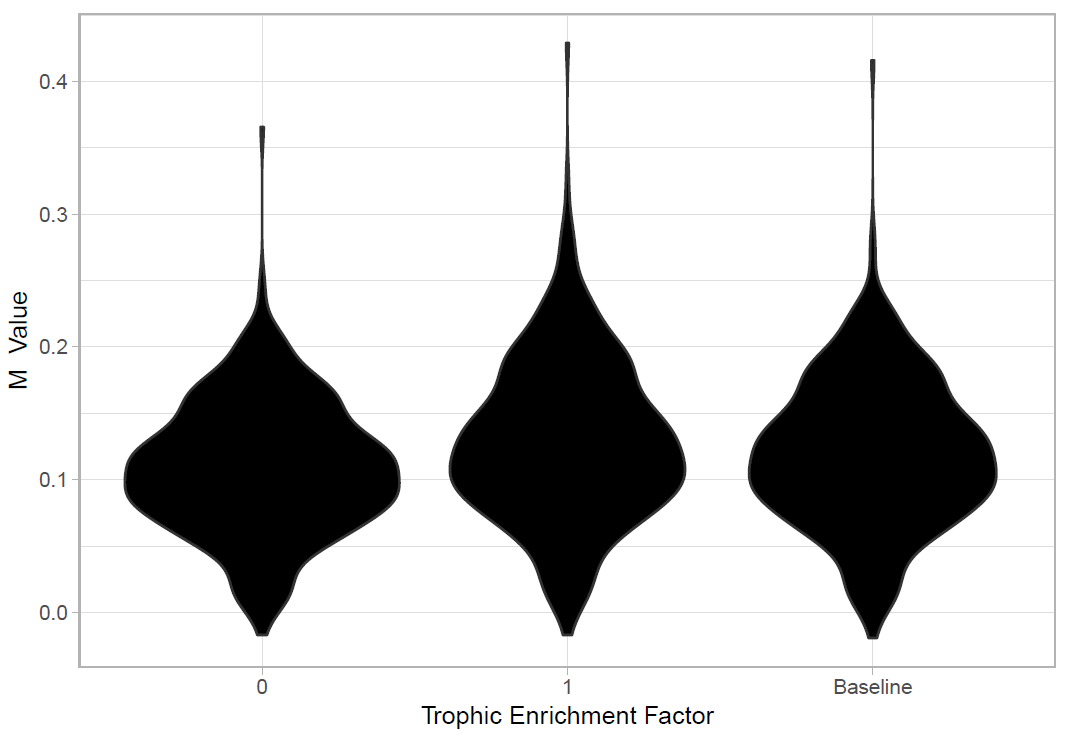
\includegraphics[width=\linewidth]{Sens_TEF.png}
\end{figure}

\begin{figure}[H]
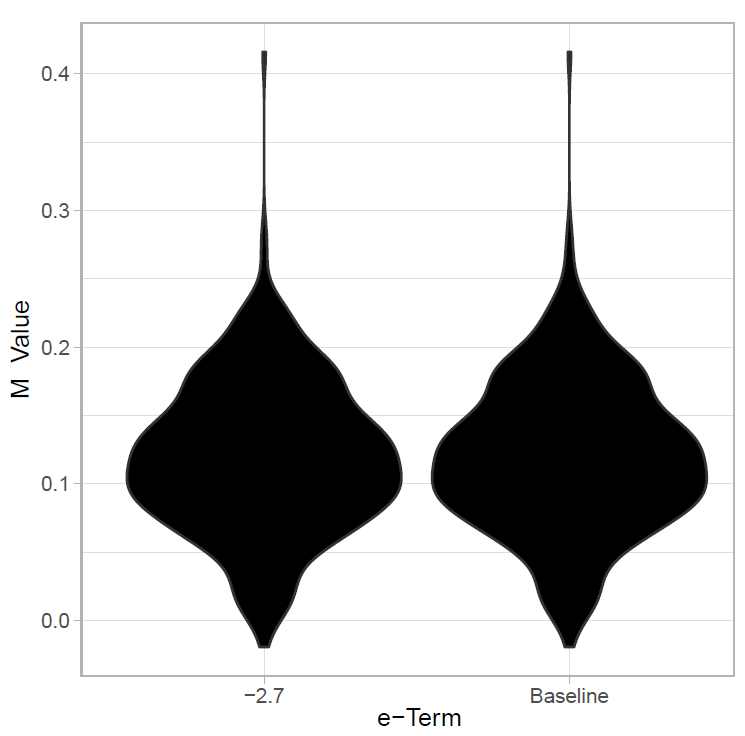
\includegraphics[width=\linewidth]{Sens_E.png}
\end{figure}

\end{document}

In this study, I used the stable isotopic composition of carbon (\textdelta \textsuperscript{13}C) in otoliths to calculate $M$.
$M$ values are proportions of the percentage of metabolic carbon in a fish's blood, which is itself a proxy for mass-specific FMR.
Otoliths are structures found within the inner ears of fishes,  made of calcium carbonate (usually aragonite) and an organic matrix. 
The carbon in otolith aragonite is derived from this metabolic carbon (dietary), and dissolved inorganic carbon, which is ingested from the surrounding seawater.
These two sources of carbon have isotopically distinct \textdelta \textsuperscript{13}C values, with \textdelta \textsuperscript{13}C from metabolic carbon being approximately 15$\permil$ higher than \textdelta \textsuperscript{13}C for dissolved inorganic carbon in most cases. % Chung 2019b
The \textdelta \textsuperscript{13}C values for an otolith is the weighted average between these two sources.
Therefore, if \textdelta \textsuperscript{13}C values of the metabolic and dissolved inorganic carbon are known, the proportion of metabolic carbon can be calculated from the \textdelta \textsuperscript{13}C value of the otolith.
A fish with a higher metabolic rate will have a higher respiration rate, and produce more metabolic carbon.
Because blood carbonate is regulated to maintain blood pH, dissolved inorganic carbon in the blood will decrease if metabolic carbon in the blood increases.
Therefore a fish with a higher metabolic rate will have a greater proportion of metabolic carbon in its blood, and in its otolith, and thus will have a higher $M$ value.






